% Long academic seminar. 37 main slides, 45 minutes; appendix excluded.
% Narrative follows IBFI 2025; paper results come from current main.tex and its inputs; slides 17--18 add IMF evidence.
% Baseline updated 18 September 2026: excludes COICOP 041 and 042; reference comparisons retain stated coverage.
\documentclass[11pt,aspectratio=169]{beamer}

\usepackage[T1]{fontenc}
\usepackage[utf8]{inputenc}
\usepackage{lmodern}
\usepackage{graphicx}
\usepackage{booktabs}
\usepackage{adjustbox}
\usepackage{amsmath}
\usepackage{xcolor}
\usepackage{ragged2e}
\usepackage{tikz}
\usepackage{colortbl}
\usetikzlibrary{calc,arrows.meta}

\definecolor{DeepNavy}{HTML}{24364B}
\definecolor{Teal}{HTML}{178C8C}
\definecolor{WarmOrange}{HTML}{E07A3F}
\definecolor{WarmGray}{HTML}{7A838C}
\definecolor{LightGray}{HTML}{E8ECEF}
\definecolor{SoftWhite}{HTML}{FFFFFF}

\setbeamertemplate{navigation symbols}{}
\setbeamertemplate{headline}{}
\setbeamertemplate{footline}{%
  \hfill\raisebox{0.6em}{\scriptsize\color{WarmGray}\insertframenumber/29}\hspace{1em}}
\setbeamertemplate{frametitle}{\vspace{.3em}\insertframetitle\par\vspace{.2em}}
\setbeamercolor{normal text}{fg=DeepNavy,bg=white}
\setbeamercolor{background canvas}{bg=white}
\setbeamercolor{frametitle}{fg=DeepNavy,bg=white}
\setbeamercolor{title}{fg=DeepNavy}
\setbeamercolor{subtitle}{fg=WarmGray}
\setbeamercolor{author}{fg=DeepNavy}
\setbeamercolor{institute}{fg=WarmGray}
\setbeamercolor{itemize item}{fg=WarmOrange}
\setbeamercolor{itemize subitem}{fg=Teal}
\setbeamerfont{frametitle}{size=\Large,series=\bfseries}
\setbeamerfont{title}{size=\LARGE,series=\bfseries}
\usefonttheme{professionalfonts}
\AtBeginDocument{\RaggedRight}

\newcommand{\source}[1]{\par\vspace{0.2em}{\scriptsize\color{WarmGray}Source: #1}}

\title{Inflation Inequality Across the Euro Area}
\author{Erwan Gautier \and J\'er\'emi Montorn\`es}
\institute{Banque de France}
\subtitle{IBFI}
\date{8 October 2026}



\pdfstringdefDisableCommands{\def\translate#1{#1}}
\setbeamertemplate{itemize item}{\small\textbullet}
\setbeamercolor{itemize item}{fg=DeepNavy}
\setbeamercolor{itemize subitem}{fg=DeepNavy}
\setbeamersize{text margin left=8mm,text margin right=8mm}

\begin{document}

% Slide 1; speaking time 0.5 min; cumulative 0.5 min.
% Evidence: Existing title
\begin{frame}[plain]
  \centering
  \vspace{0.20\textheight}
  {\LARGE\bfseries Inflation Inequality Across the Euro Area\par}
  \vspace{1.2em}
  {\large Erwan Gautier \qquad J\'er\'emi Montorn\`es\par}
  \vspace{0.6em}
  {\normalsize Banque de France\par}
  \vspace{0.6em}
  {\normalsize IBFI\par}
  \vspace{0.6em}
  {\normalsize 8 October 2026\par}
\end{frame}

% Slide 2; speaking time 1 min; cumulative 1.5 min.
% Evidence: main.tex, introduction
\begin{frame}{Household Inflation Exposure in the Euro Area}
\begin{itemize}
\item How do relative-price shocks affect households with different consumption baskets?
\item Construct monthly inflation indices by income, age and residence for 20 euro-area countries, excluding rents, calibrated to HICP weights on matched products.
\item Counterfactual price paths quantify how fiscal measures changed average inflation and income-group gaps.
\item Household microdata reveal the dispersion concealed by group averages.
\end{itemize}
\end{frame}

% Slide 3; speaking time 1.5 min; cumulative 3 min.
% Evidence: Promoted from appendix: three channels, retained
\begin{frame}{What Our Inflation Indices Capture}
\centering
\small
\renewcommand{\arraystretch}{1.7}
\setlength{\tabcolsep}{6pt}
\begin{tabular}{@{}>{\RaggedRight\arraybackslash}p{0.23\textwidth}>{\RaggedRight\arraybackslash}p{0.53\textwidth}>{\centering\arraybackslash}p{0.15\textwidth}@{}}
\toprule
\textbf{Channel} & \textbf{Mechanism} & \textbf{Covered here?}\\
\midrule
Consumption baskets & Different expenditure shares imply different inflation exposure & \textcolor{Teal}{\textbf{Yes}}\\
Nominal income & Wages, pensions and transfers adjust to inflation & No\\
Balance sheets & Unexpected inflation revalues nominal assets and debt; asset prices may also adjust & No\\
\bottomrule
\end{tabular}
\par\vspace{.5em}\raggedright\small
Different inflation rates do not by themselves rank households' welfare losses.
\end{frame}

% Slide 4: Prices Paid Within Product Categories Remain Unobserved
% Evidence: main.tex, literature discussion; narrative from supplied PPTX, without legacy numerical results
\begin{frame}{Prices Paid Within Product Categories Remain Unobserved}
\noindent{\small Household microdata reveal different baskets; scanner data additionally reveal detailed product choices and transaction prices.\par}\vspace{.6em}
\small
\begin{tabular}{@{}>{\RaggedRight\arraybackslash}p{.25\textwidth}>{\RaggedRight\arraybackslash}p{.49\textwidth}>{\RaggedRight\arraybackslash}p{.18\textwidth}@{}}
\toprule
Source of heterogeneity & Example & Our indices\\
\midrule
Across categories & Different shares of food, energy and services & Captured\\[.6em]
Within categories & Different brands, pack sizes or organic vs.\ regular products & Not observed\\[.6em]
Within identical products & Different retailers, promotions or purchase dates & Not observed\\
\bottomrule
\end{tabular}


\end{frame}

% Slide 5; speaking time 1 min; cumulative 4 min.
% Evidence: main.tex, introduction; annual country and product tables; burden section
\begin{frame}{Main Findings, 2021--2023}
\begin{itemize}
\item The annual Q1--Q5 inflation gap reached \textbf{1.2 percentage points in 2022}, with large differences across countries.
\item Price policies lowered inflation by \textbf{1.4 points in 2022} and reduced the income gap by \textbf{0.5 point}.
\item Household characteristics explain only a small part of inflation dispersion within countries.
\item In 2022, scaled inflation exposure was \textbf{12.3\% of income for Q1}, against \textbf{6.1\% for Q5}, using 2020 expenditure-to-income ratios.
\end{itemize}
\vspace{.5em}
\end{frame}

% Slide 6; speaking time 1 min; cumulative 4 min.
% Evidence: Existing illustrative example, explicitly not an estimate
\begin{frame}{An introductory example}
\noindent{\small Different baskets generate an inflation gap only when price changes differ across products.\par}
\vspace{.7em}
\centering
\small
\renewcommand{\arraystretch}{1.5}
\setlength{\tabcolsep}{4pt}
\begin{tabular}{@{}>{\RaggedRight\arraybackslash}p{.11\textwidth}>{\RaggedRight\arraybackslash}p{.34\textwidth}>{\centering\arraybackslash}p{.15\textwidth}>{\centering\arraybackslash}p{.15\textwidth}>{\centering\arraybackslash}p{.16\textwidth}@{}}
\toprule
& \textbf{Expenditure share} & \textbf{First quintile}\newline of income & \textbf{Fifth quintile}\newline of income & \textbf{Inflation gap}\newline (Q1--Q5)\\
\midrule
& Housing energy & 10\% & 6\% & --\\
& Other consumption & 90\% & 94\% & --\\
\midrule
\textbf{Shock 1} & \textbf{Energy prices +40\%}\newline Other prices unchanged & \textbf{4.0\%} & \textbf{2.4\%} & \textcolor{Teal}{\textbf{1.6 pp}}\\[.4em]
\midrule
\textbf{Shock 2} & \textbf{All prices +40\%}\newline Energy and other consumption & \textbf{40.0\%} & \textbf{40.0\%} & \textcolor{Teal}{\textbf{0.0 pp}}\\[.4em]
\bottomrule
\end{tabular}
\end{frame}

% Slide 7; speaking time 1.5 min; cumulative 5.5 min.
% Evidence: main.tex, figure hicp
\begin{frame}{Energy and Food Drove Large Relative-Price Changes}
\noindent{\small Euro area, year-on-year inflation (\%).\par}\vspace{.4em}
\centering
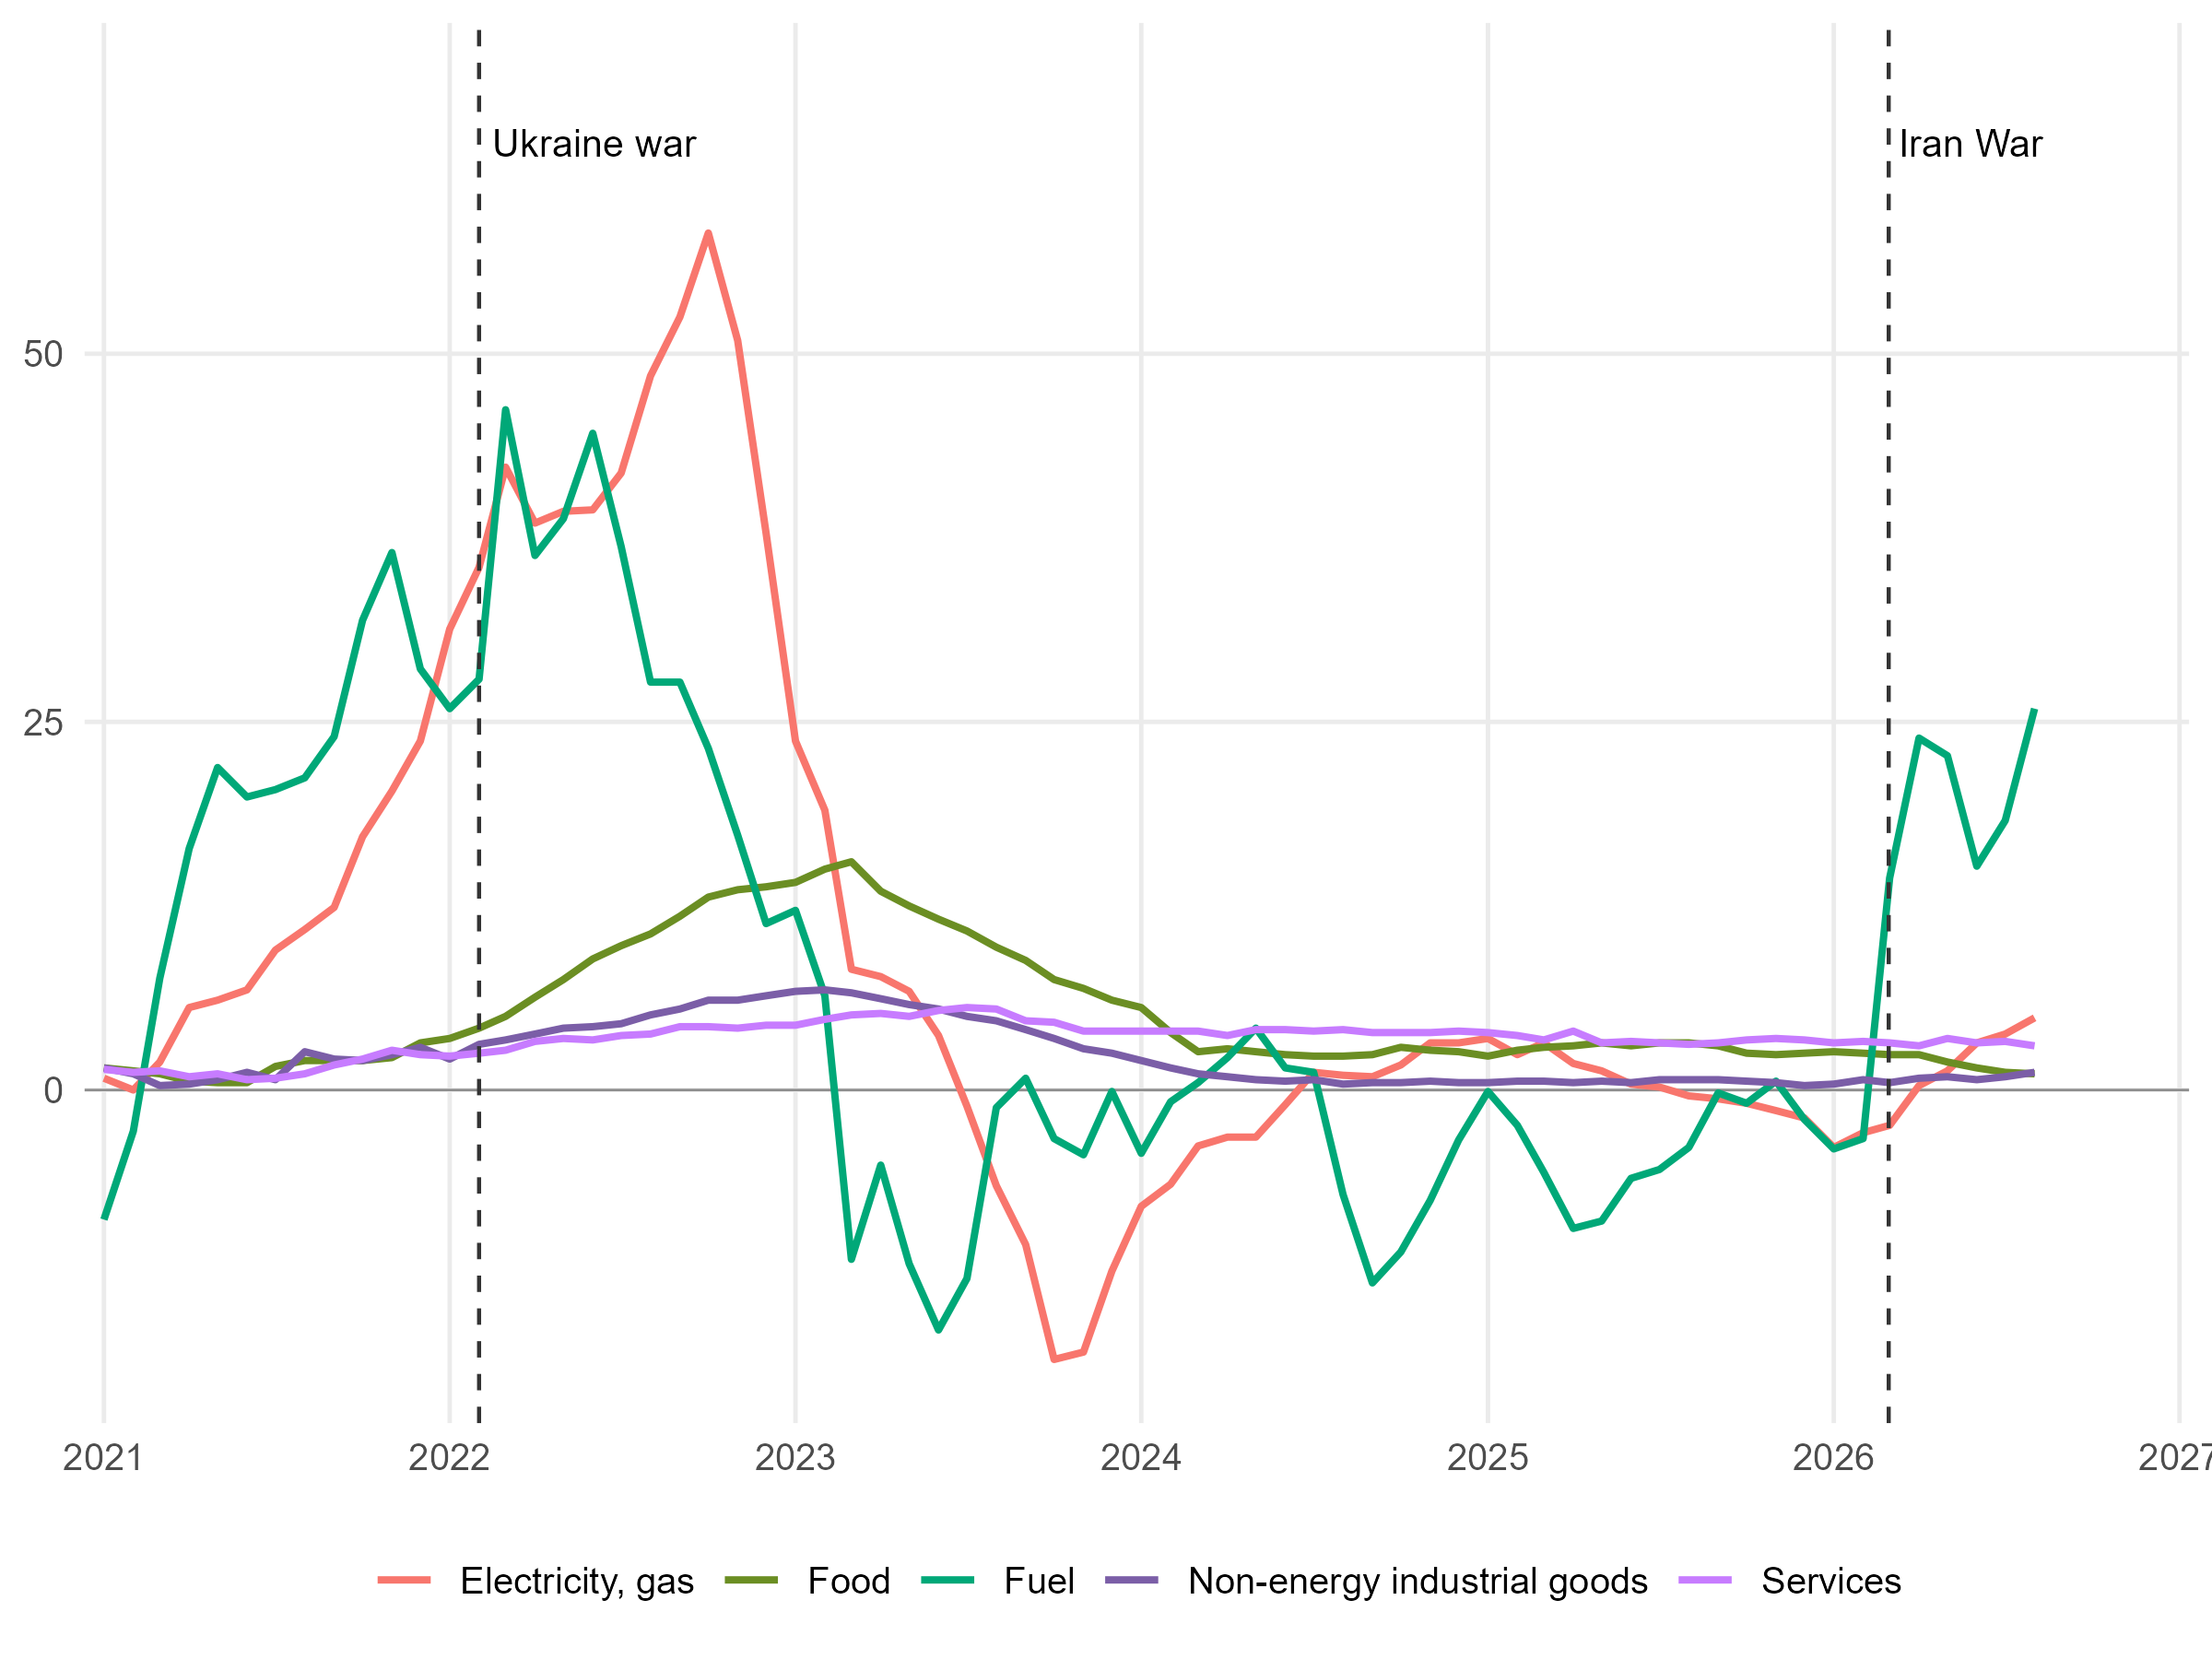
\includegraphics[width=.94\textwidth,height=.65\textheight,keepaspectratio]{fig/fig_EA_2014_2026_hicp_components.png}
\source{Eurostat HICP and HBS; authors\textquotesingle\ calculations.}
\end{frame}

% Slide 8; speaking time 1.5 min; cumulative 7 min.
% Evidence: main.tex, figure hbs
\begin{frame}{Consumption Baskets Differ Across Income Quintiles}
\noindent{\small Shares of total expenditure including rents, 2020 (\%).\par}\vspace{.4em}
\centering
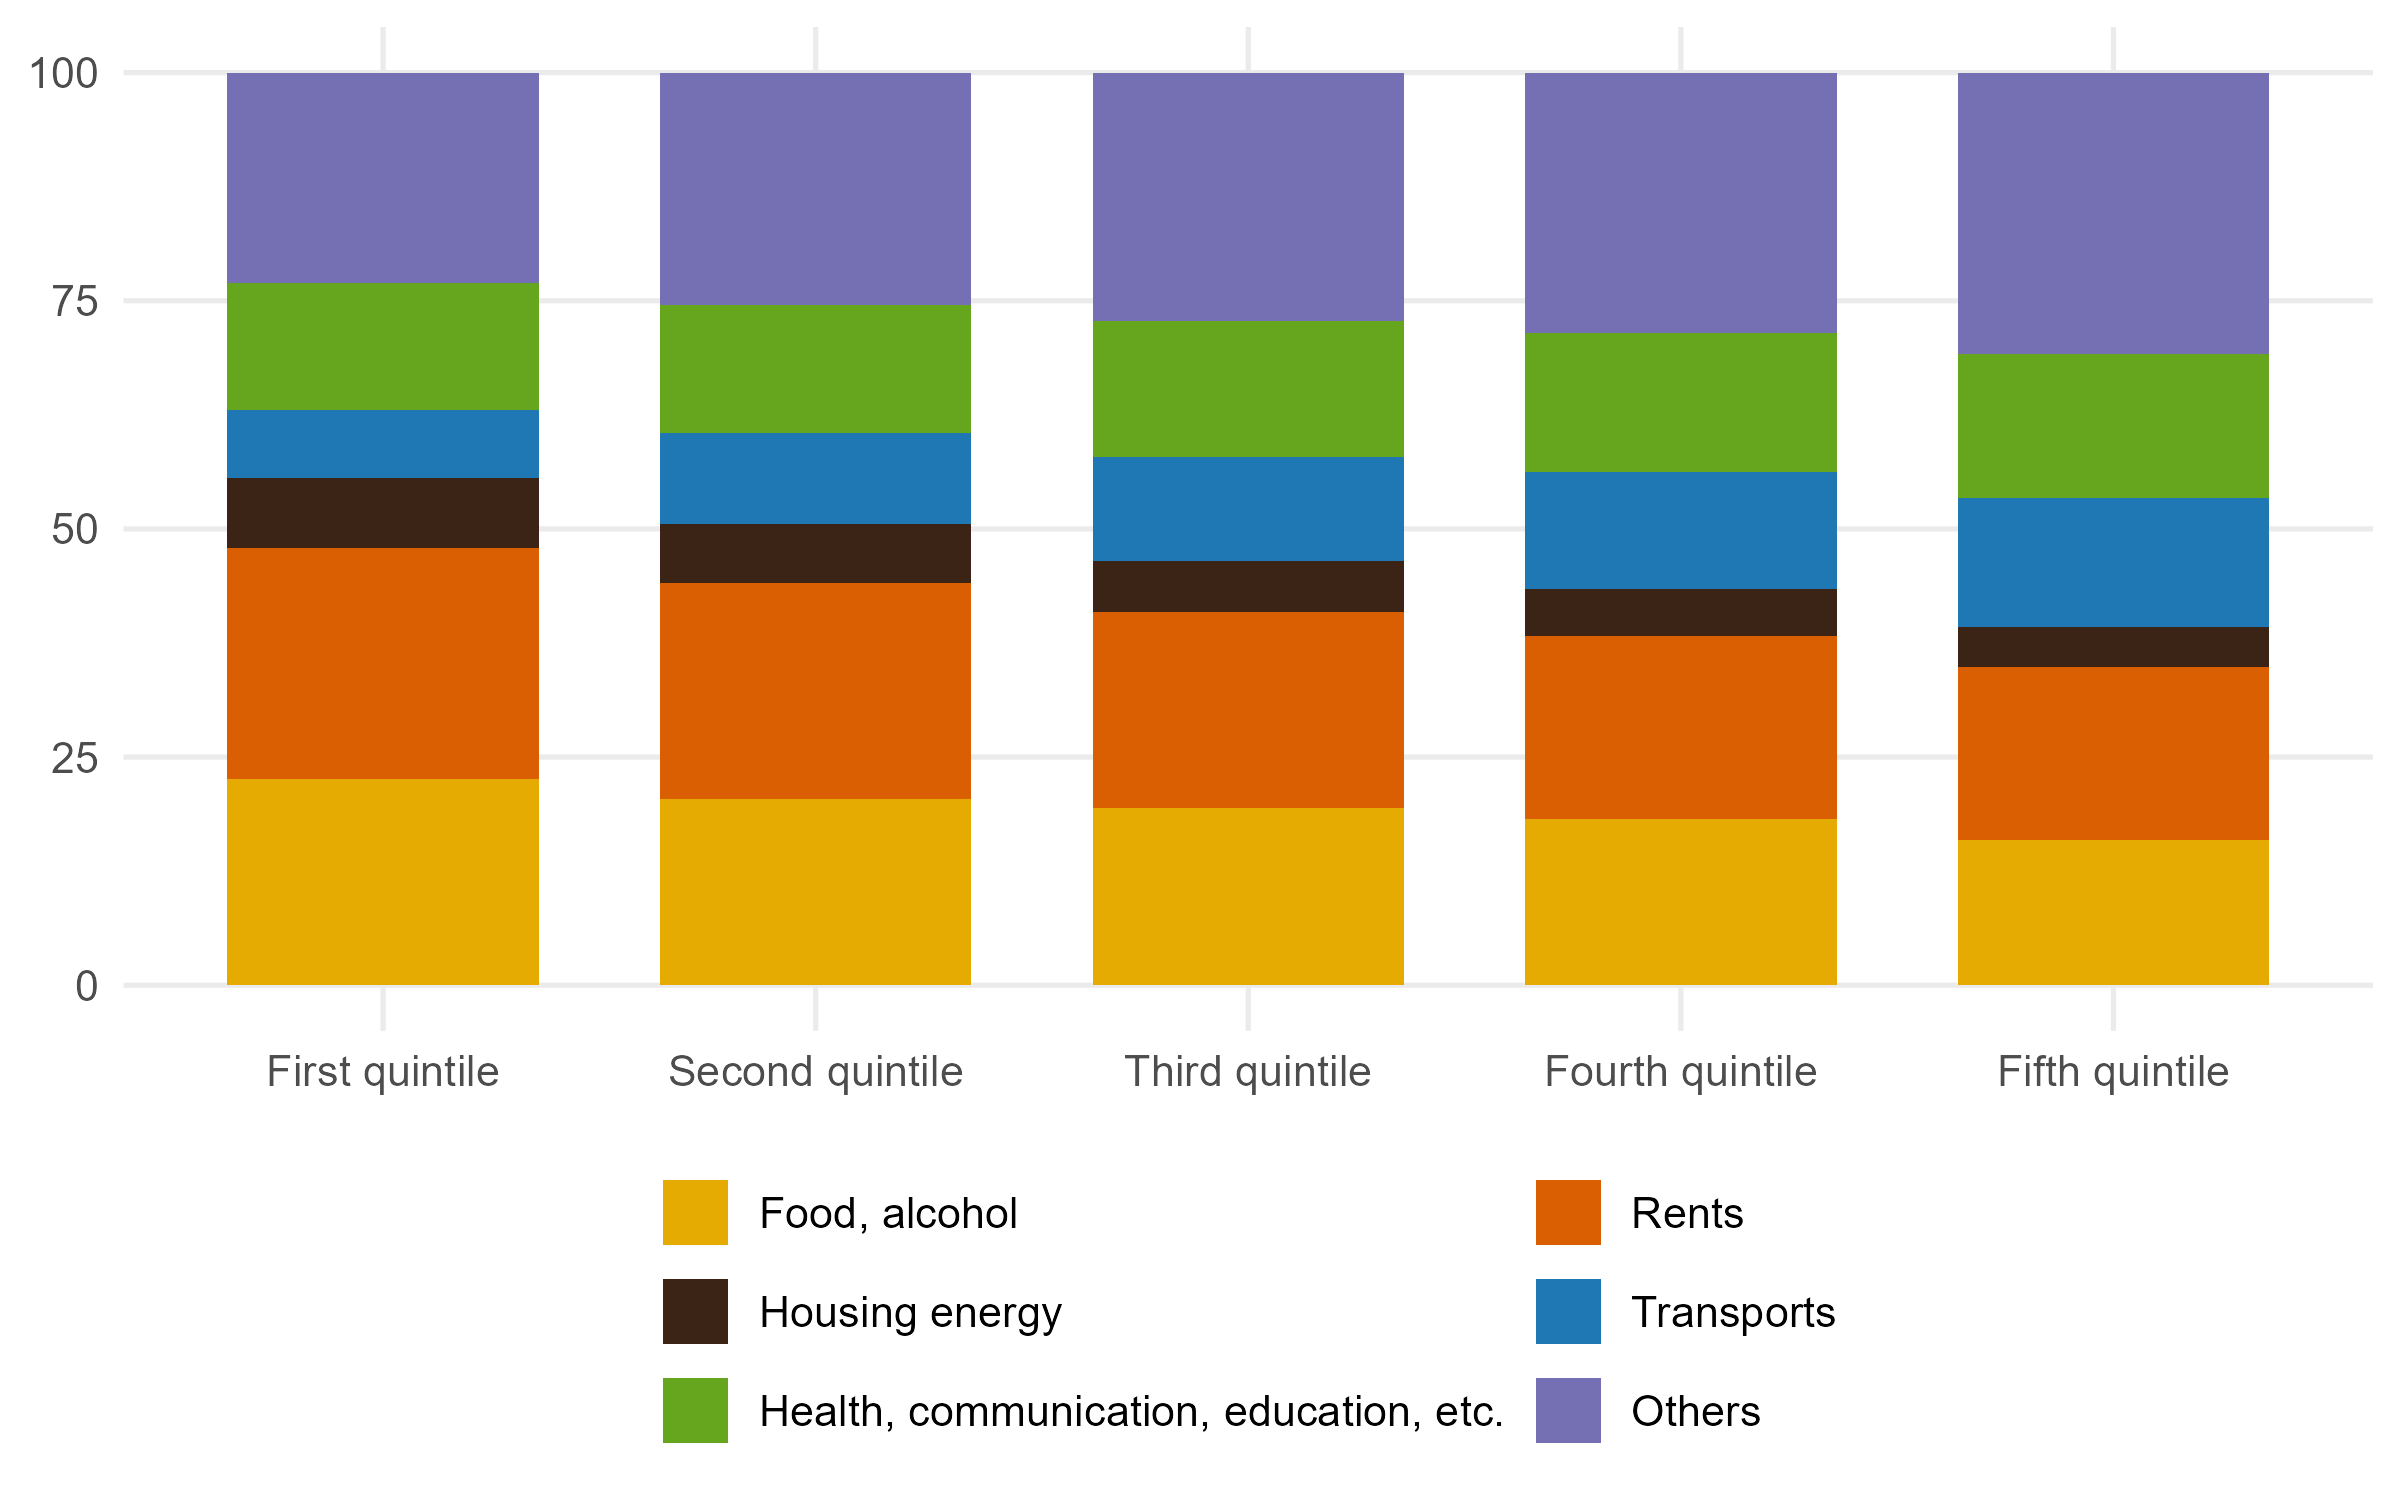
\includegraphics[width=.94\textwidth,height=.65\textheight,keepaspectratio]{fig/fig_EA_2020_income_consumption_baskets.png}
\source{Eurostat HICP and HBS; authors\textquotesingle\ calculations.}
\end{frame}

% Slide 9; speaking time 1 min; cumulative 8 min.
% Evidence: main.tex, data and methodology
\begin{frame}{Linking HICP Prices to Household Budget Surveys}
\begin{itemize}
\item \textbf{Prices:} monthly HICP component indices and annual official product weights.
\item \textbf{Baskets:} HBS expenditure profiles by income, age and residence, usually observed every five years.
\item \textbf{Matching:} harmonized three-digit COICOP categories across 20 countries; national HBS sources supplement Italy.
\item \textbf{Coverage:} exclude actual and imputed rents (041, 042), then renormalize. Within-product prices and substitution are unobserved.
\end{itemize}
\end{frame}

% Slide 10; speaking time 1 min; cumulative 9 min.
% Evidence: main.tex, group price indices
\begin{frame}{Monthly and Annual Inflation Use Chained Indices}
Within each year, prices are compared with the preceding December:
\[
P_{g,y,m}=\sum_j\omega_{j,g,y}\frac{p_{j,y,m}}{p_{j,y-1,12}},
\qquad I_{g,y,m}=I_{g,y-1,12}P_{g,y,m}.
\]
\begin{itemize}
\item Monthly figures: year-on-year changes in $I_{g,y,m}$.
\item Annual tables: percentage change in the annual-average index.
\item Euro-area indices: aggregation with annual HICP country weights.
\end{itemize}
\vspace{.4em}
The annual Q1--Q5 gap is the difference between the two annual inflation rates, in percentage points.

\end{frame}

% Slide 11; speaking time 1 min; cumulative 10 min.
% Evidence: main.tex, group weights and RAS appendix
\begin{frame}{Group Baskets Aggregate to Official HICP Weights}
Let $s_{g,y}$ be group $g$'s share of total consumption and
$\bar\omega^{\mathrm{HICP}}_{j,y}$ the official product share on matched non-rent products.
\vspace{.5em}
\[
\sum_j M_{j,g,y}=s_{g,y},\qquad
\sum_g M_{j,g,y}=\bar\omega^{\mathrm{HICP}}_{j,y}.
\]
RAS adjusts the product-by-group expenditure matrix $M$ to match both margins.
\[
\omega_{j,g,y}=\frac{M_{j,g,y}}{s_{g,y}},\qquad
\sum_g s_{g,y}\omega_{j,g,y}=\bar\omega^{\mathrm{HICP}}_{j,y}.
\]
\textbf{The calibration uses expenditure shares, not population shares.}
\end{frame}



% Slide 12; speaking time 1 min; cumulative 11 min.
% Evidence: main.tex, short-run income figure
\begin{frame}{The Income Inflation Gap Peaked During the Energy Shock}
\noindent{\small\color{WarmGray}ECB analysis reports similar findings using a slightly different methodology (Bobasu et al., 2023).\par}
\vspace{0.3em}
\centering
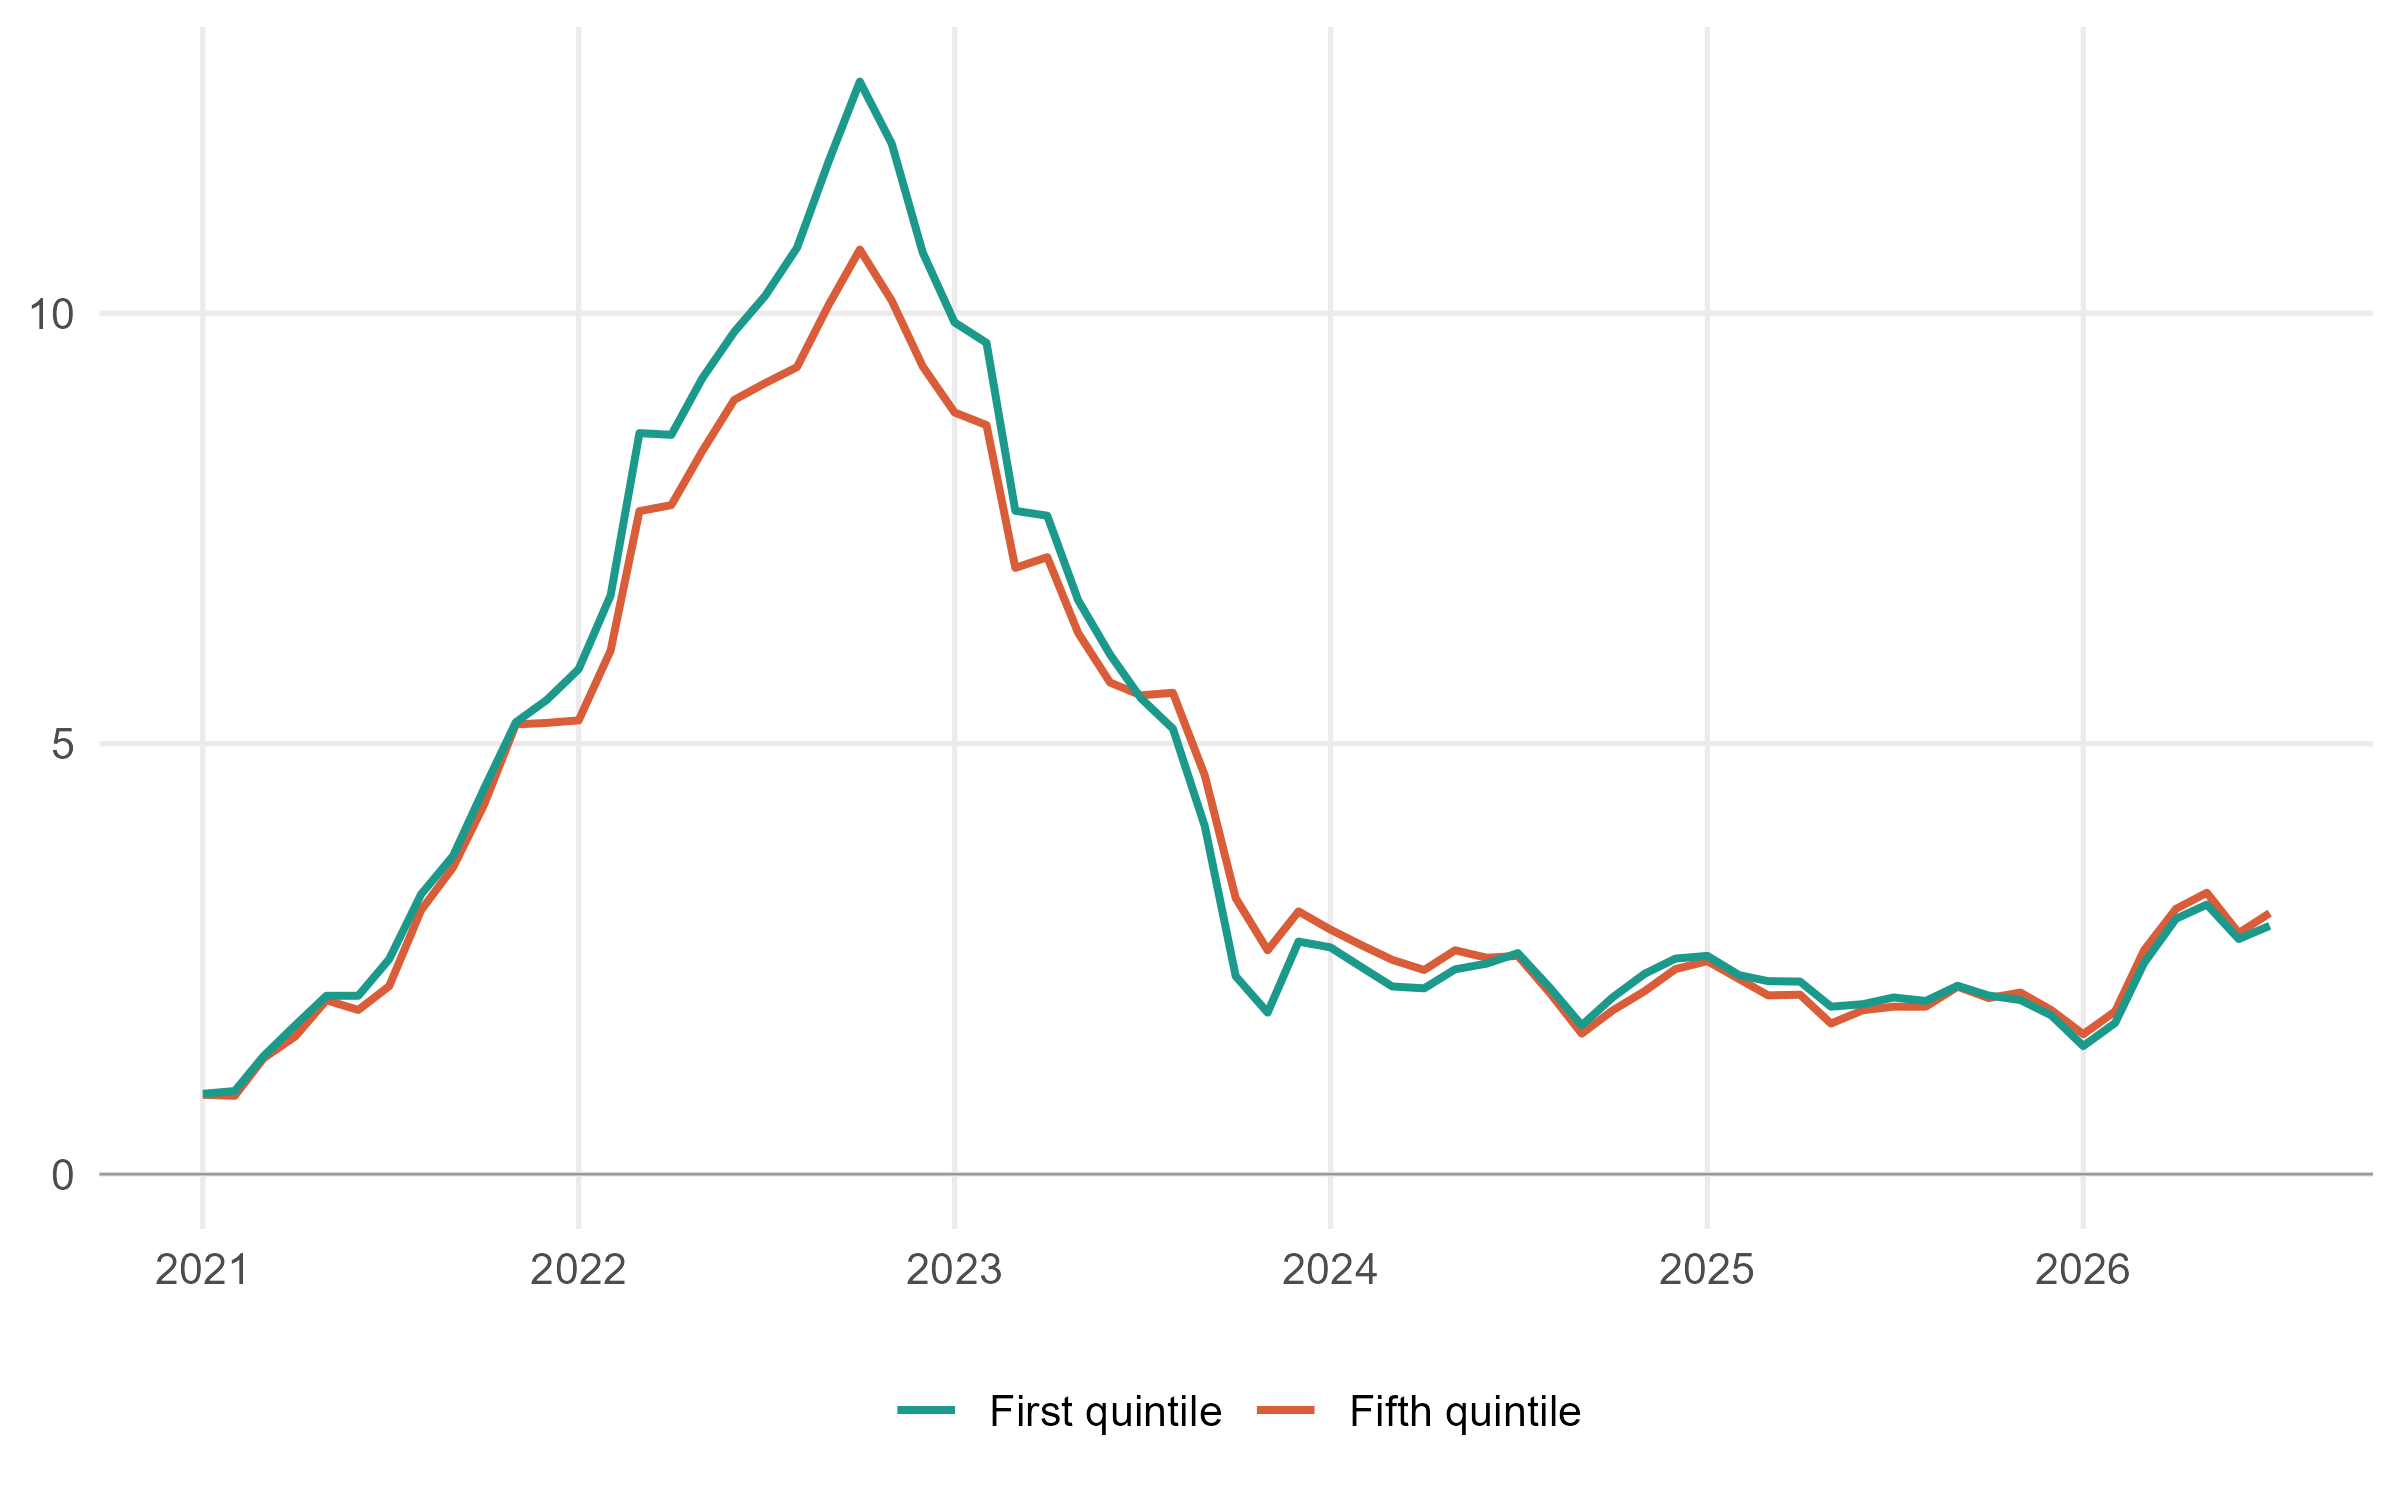
\includegraphics[width=0.82\textwidth,height=0.57\textheight,keepaspectratio]{fig/fig_EA20_2020_2026_income_inflation_Q1_Q5.png}
\source{Eurostat HICP and HBS; authors' calculations. Units: year-on-year inflation, in percent.}
\raggedright
\par\vspace{.5em}
{\small Calculate and visualize inflation inequality with our R package:\par
\href{https://github.com/JeremiMontornes/inflationinequality}{\textcolor{Teal}{github.com/JeremiMontornes/inflationinequality}}\par}
\end{frame}

% Slide 13; speaking time 1.5 min; cumulative 12.5 min.
% Evidence: tables/tab_EA20_country_income_q1_q5_cumulative_gap_2021_06_2023_06.tex
\begin{frame}{National Income Gaps Differed in Magnitude and Sign}
\centering
\small\renewcommand{\arraystretch}{1.2}
\begin{tabular}{lrrr}
\toprule
Q1--Q5 gap (pp) & 2021 & 2022 & 2023\\
\midrule
Latvia & -0.2 & 4.8 & 2.5\\
Estonia & 0.5 & 4.4 & 1.3\\
Ireland & 0.5 & 3.0 & 1.1\\
Italy & 0.1 & 1.6 & 0.5\\
Germany & -0.4 & 1.4 & 0.6\\
France & 0.3 & 0.2 & 0.2\\
Finland & -0.2 & -0.9 & 0.4\\
\midrule
\textbf{Euro area} & \textbf{0.1} & \textbf{1.2} & \textbf{0.1}\\
\bottomrule
\end{tabular}
\end{frame}

% Slide 14; speaking time 1.5 min; cumulative 14 min.
% Evidence: main.tex, observed product decomposition
\begin{frame}{Household Energy and Food Widened the Income Gap}
\noindent{\small\color{WarmGray}The distributional impact of inflation depends on which prices rise, as well as on the size of the aggregate shock.\par}
\vspace{0.5em}
\centering
\footnotesize
\setlength{\tabcolsep}{7pt}
\begin{tabular}{l*{3}{>{\centering\arraybackslash}p{1.8cm}}}
\toprule
& \multicolumn{3}{c}{Q1--Q5 inequality contribution}\\
\cmidrule(lr){2-4}
Product group & 2021 & 2022 & 2023\\
\midrule
Food and non-alcoholic beverages & 0.1 & 0.7 & 0.7\\
Alcohol, tobacco and narcotics & 0.1 & 0.1 & 0.2\\
Clothing and footwear & 0.0 & 0.0 & -0.1\\
Housing maintenance and furnishings & -0.1 & -0.3 & -0.2\\
Housing energy & 0.4 & 1.8 & 0.1\\
Operation of personal transport equipment & -0.3 & -0.4 & 0.0\\
Transport (excluding vehicle operation) & -0.1 & -0.3 & -0.2\\
Other & -0.1 & -0.5 & -0.5\\
\midrule
\textbf{Total} & \textbf{0.1} & \textbf{1.2} & \textbf{0.1}\\
\bottomrule
\end{tabular}
\vspace{0.5em}


\source{Eurostat HICP and HBS; authors' calculations. Product rows are contributions to the Q1--Q5 annual inflation-rate gap, in percentage points.}
\end{frame}

% Slide 15; speaking time 1.5 min; cumulative 18.5 min.
% Evidence: IMF Fiscal Monitor April 2023, chapter 2, Figure 2.5 and channel discussion.
\begin{frame}{Focus: Kenya and Senegal}
\noindent{\small Kenya and Senegal, 2021Q2--2022Q2; inflation by quintile (\%).\par}
\centering
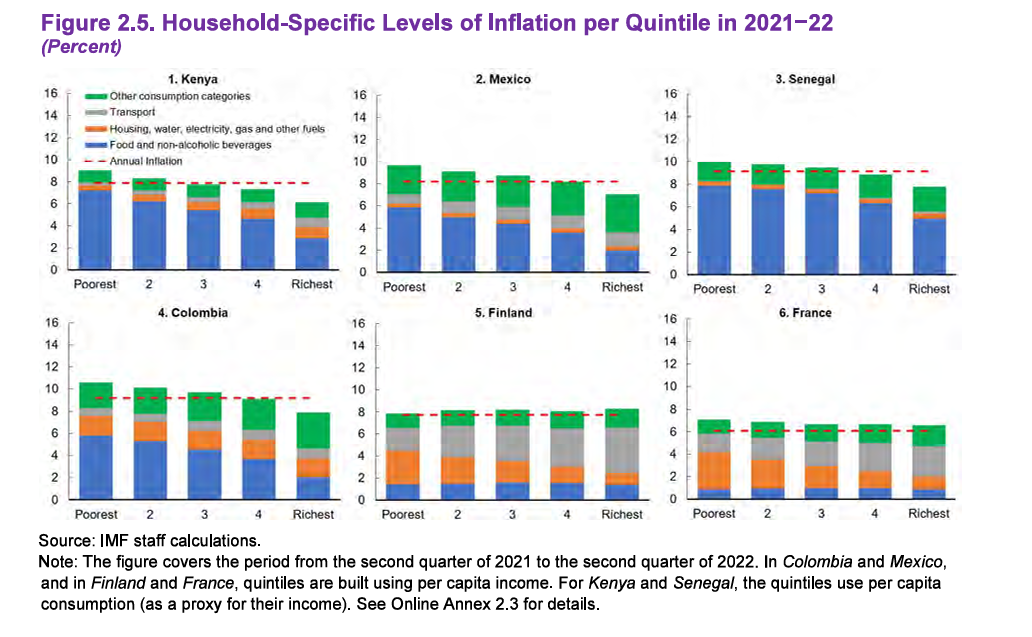
\includegraphics[height=.47\textheight,trim=40bp 339bp 680bp 60bp,clip]{fig/imf_fm2023_figure2_5.png}\hspace{.8em}
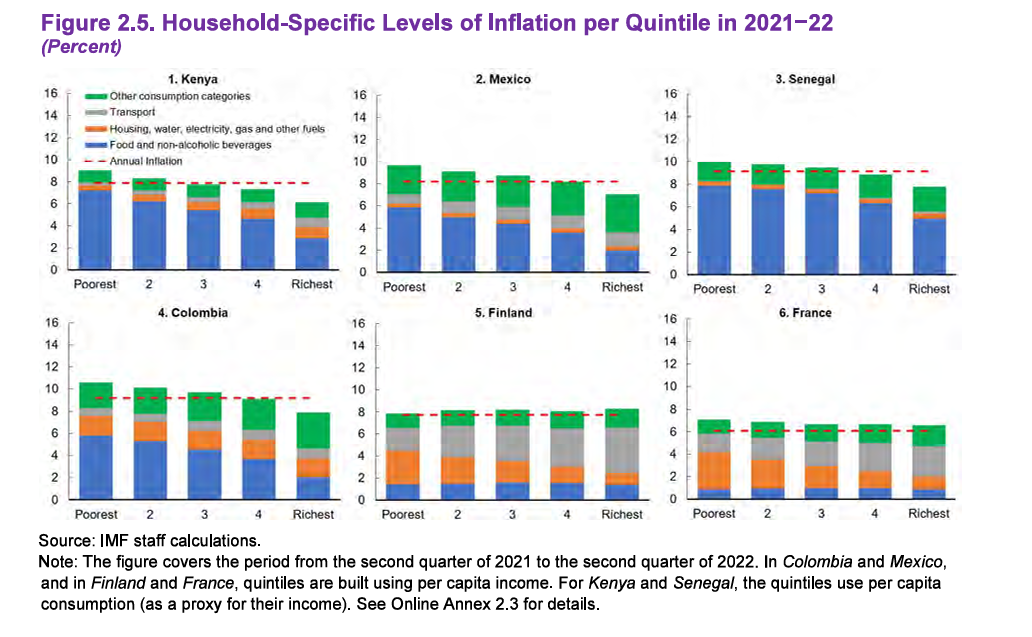
\includegraphics[height=.47\textheight,trim=662bp 339bp 70bp 60bp,clip]{fig/imf_fm2023_figure2_5.png}
\par\smallskip\raggedright\small
\begin{itemize}
\item Faster food-price increases weigh more on poorer households because food absorbs a larger share of their spending.
\item In Kenya and Senegal, nominal incomes also failed to keep pace with prices.
\end{itemize}
\source{\href{https://www.imf.org/en/-/media/files/publications/fiscal-monitor/2023/april/english/ch2.pdf}{IMF, Fiscal Monitor, April 2023, ch.\ 2, Fig.\ 2.5 and discussion}. Quintiles: per-capita consumption. Dashed lines: national inflation.}
\end{frame}

% Slide 16; speaking time 1.5 min; cumulative 20 min.
% Evidence: same IMF source; euro-area benchmark from main.tex.
\begin{frame}{Focus: Mexico and Colombia}
\noindent{\small Mexico and Colombia, 2021Q2--2022Q2; inflation by quintile (\%).\par}
\centering
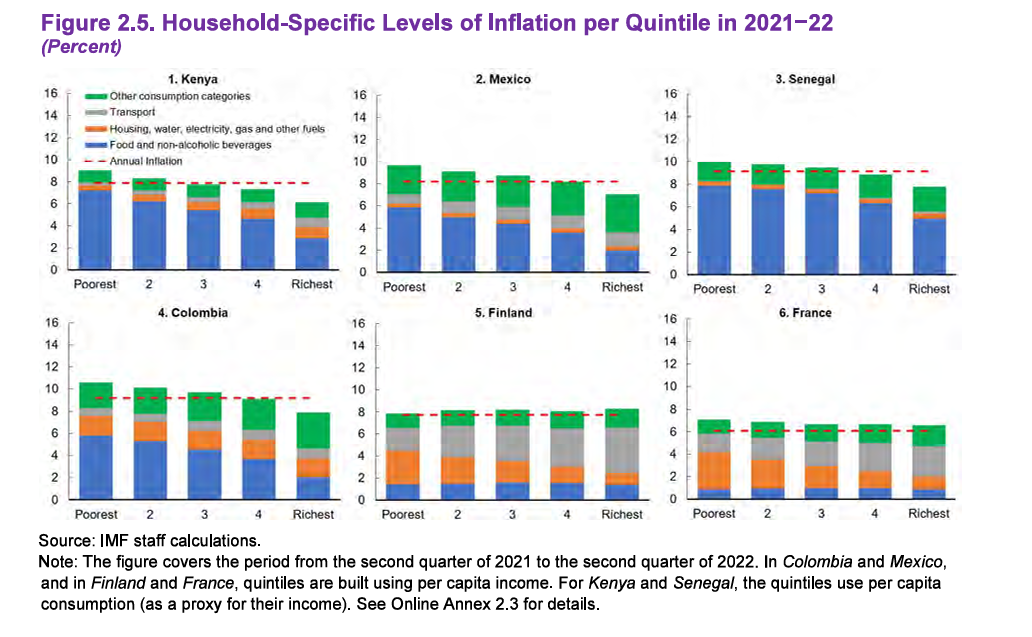
\includegraphics[height=.39\textheight,trim=344bp 339bp 377bp 60bp,clip]{fig/imf_fm2023_figure2_5.png}\hspace{.8em}
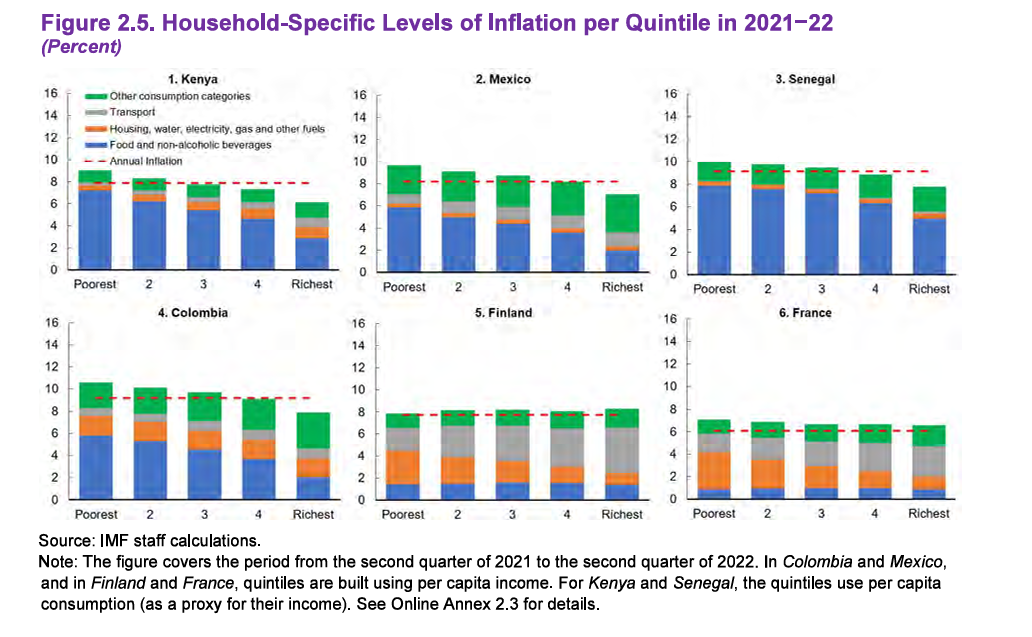
\includegraphics[height=.39\textheight,trim=40bp 114bp 680bp 300bp,clip]{fig/imf_fm2023_figure2_5.png}
\par\smallskip\raggedright\small
\begin{itemize}
\item Food also drives the income gradient here, but real incomes rose. Income and wealth effects can outweigh basket exposure.
\item Basket gaps can narrow or reverse as relative prices change.
\end{itemize}
\par\smallskip\footnotesize
Euro-area benchmark: Q1--Q5 = \textbf{1.2 pp in calendar 2022}. Periods and quintiles differ: the IMF uses per-capita income here; our groups use total household income.
\source{\href{https://www.imf.org/en/-/media/files/publications/fiscal-monitor/2023/april/english/ch2.pdf}{IMF, Fiscal Monitor, April 2023, ch.\ 2, Fig.\ 2.5 and discussion}; euro area: this paper. Colors as on previous slide; dashed lines: national inflation.}
\end{frame}

% Slide 17; speaking time 1.5 min; cumulative 21.5 min.
% Evidence: main.tex, constructing counterfactual price indices
\begin{frame}{Euro area: Fiscal Measures Directly Reduced\\Consumer Prices}
\begin{itemize}
\item \textbf{Administered prices:} electricity and gas tariff shields, retail caps and regulated charges.
\item \textbf{Tax reductions:} temporary VAT and excise cuts on energy and selected food products.
\item \textbf{Unit support:} fuel rebates and per-kWh subsidies.
\end{itemize}
\vspace{.7em}
Price-based support in the inventory totals \textbf{EUR 268.9 billion}:
EUR 236.2 billion untargeted and EUR 32.8 billion targeted.
\end{frame}

% Slide 18; speaking time 2 min; cumulative 25 min.
% Evidence: French counterfactual definitions retained from slides.tex; gas, electricity and motor fuels.
\begin{frame}{France: Defining the Energy-Price Counterfactuals}
\scriptsize\setlength{\abovedisplayskip}{1pt}\setlength{\belowdisplayskip}{1pt}\setlength{\abovedisplayshortskip}{2pt}\setlength{\belowdisplayshortskip}{2pt}
\textcolor{WarmGray}{$CF$ = counterfactual; $O$ = observed; $TRV_{\mathrm{gas}}$: gas tariff (EUR/kWh); $TRV_e$: electricity tariff (EUR/kWh).}\par
\par\vspace{0.5em}
\begin{columns}[T,onlytextwidth]
\begin{column}{0.48\textwidth}
\textcolor{Teal}{\textbf{1. Gas \enspace  Nov. 2021--June 2023}}
\[
\Delta P_{\mathrm{gas},t}^{CF}=\beta_{\mathrm{gas}}\,\Delta TRV_{\mathrm{gas},t}^{CF}
\]
{\color{WarmGray}unit-free decimal rates.}\par

$\beta_{\mathrm{gas}}=0.82$.
\par\vspace{0.5em}
\textcolor{Teal}{\textbf{3. Motor fuels \enspace  Apr.--Dec. 2022}}
\[
p_{\mathrm{fuel},t}^{CF}=p_{\mathrm{fuel},t}^{O}+r_t
\qquad\text{(EUR/litre, incl. taxes)}
\]
Chained index:
\[
P_{\mathrm{fuel},t}^{CF}=P_{\mathrm{fuel},t-1}^{CF}
\frac{p_{\mathrm{fuel},t}^{O}+r_t}{p_{\mathrm{fuel},t-1}^{O}+r_{t-1}}.
\]
Monthly rebates (EUR/litre):
\par\smallskip
\begin{tabular}{@{}lr@{\qquad}lr@{}}
Apr.--Aug. & $r=0.18$ & Sept.--Oct. & $r=0.30$\\
November & $r=0.22$ & December & $r=0.10$
\end{tabular}
\par\smallskip

\end{column}
\begin{column}{0.49\textwidth}
\textcolor{Teal}{\textbf{2. Electricity \enspace  Feb. 2022--Feb. 2024}}
\[
\Delta P_{e,t}^{CF}=\beta_e\,\Delta TRV_{e,t}^{CF}
\]
{\color{WarmGray}unit-free decimal rates.}\par

$\beta_e=1.02$.
\par\smallskip
\begin{tabular}{@{}lll@{}}
\toprule
Date & Observed reference & $\Delta TRV_{e,t}^{CF}$\\
\midrule
Feb. 2022 & Jan. 2022 & $33.24\%$\\
Feb. 2023 & Jan. 2023 & $108.91\%$\\
Feb. 2024 & Feb. 2024 & $0\%^{\dagger}$\\
\bottomrule
\end{tabular}
\par\smallskip

\par\smallskip

\par\smallskip
$^{\dagger}$Model closure, not a tariff estimate: $P_{e,t}^{CF}=P_{e,t}^{O}$.
\end{column}
\end{columns}

\end{frame}

% Slide 19; speaking time 1 min; cumulative 26 min.
% Evidence: Promoted from appendix; French component paths
\begin{frame}{France: Observed and Counterfactual Energy Price Indices}
\noindent{\small\color{WarmGray}January 2020 = 100; January 2020--June 2026. Vertical scales differ across panels.\par}
\vspace{0.5em}
\centering
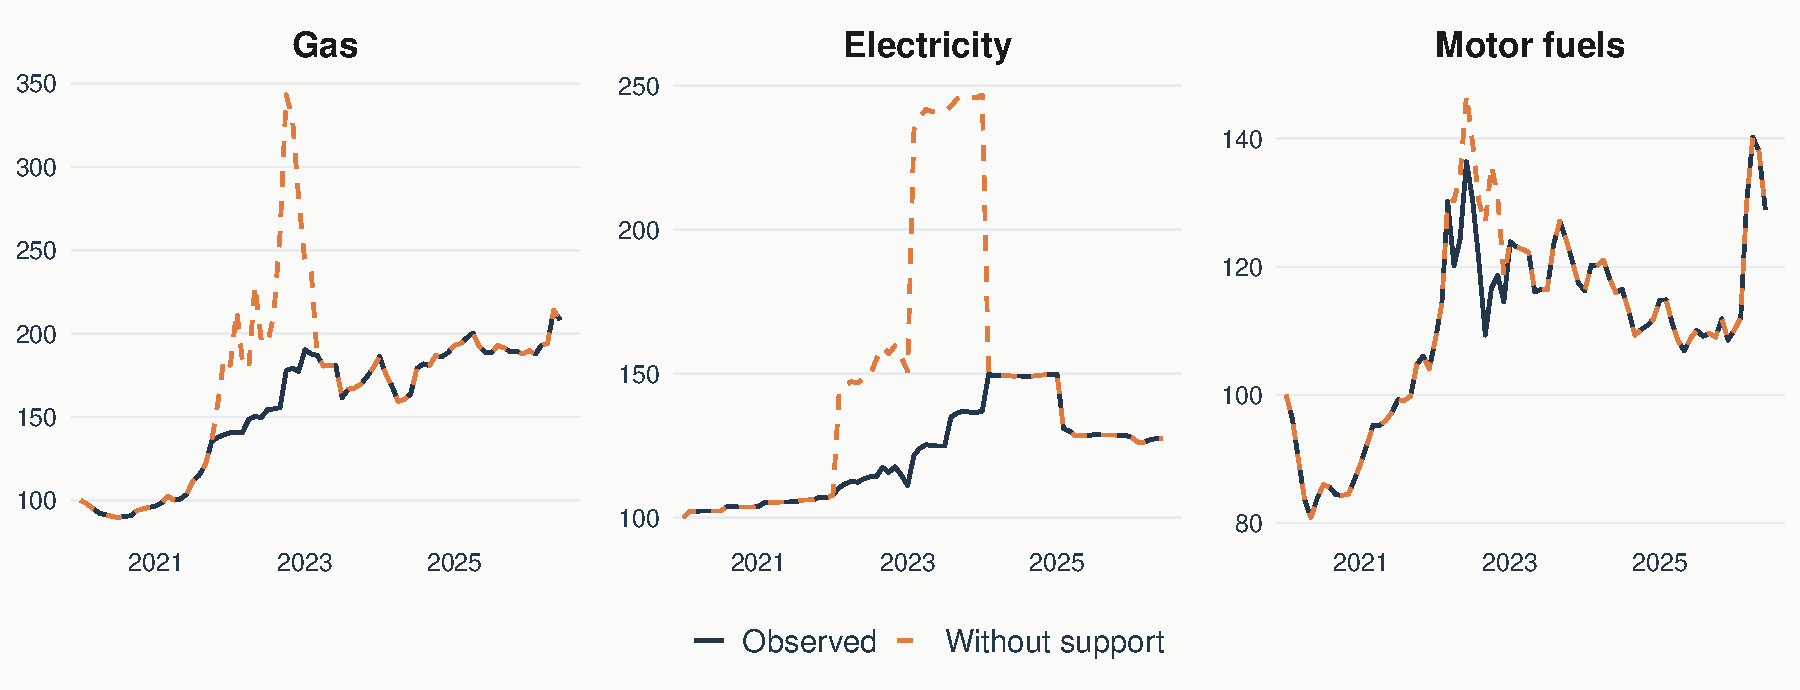
\includegraphics[width=\textwidth,height=0.69\textheight,keepaspectratio]{fig/slide_fr_energy_price_indices.pdf}
\source{French observed and no-policy component price series; authors' calculations.}
\end{frame}

% Slide 20; speaking time 1.5 min; cumulative 27.5 min.
% Evidence: main.tex, total policy inflation figure; original chart without overlay
\begin{frame}{Price Policies Compressed the Inflation Peak}
\noindent{\small Observed and no-policy year-on-year inflation (\%).\par}\vspace{.4em}
\centering
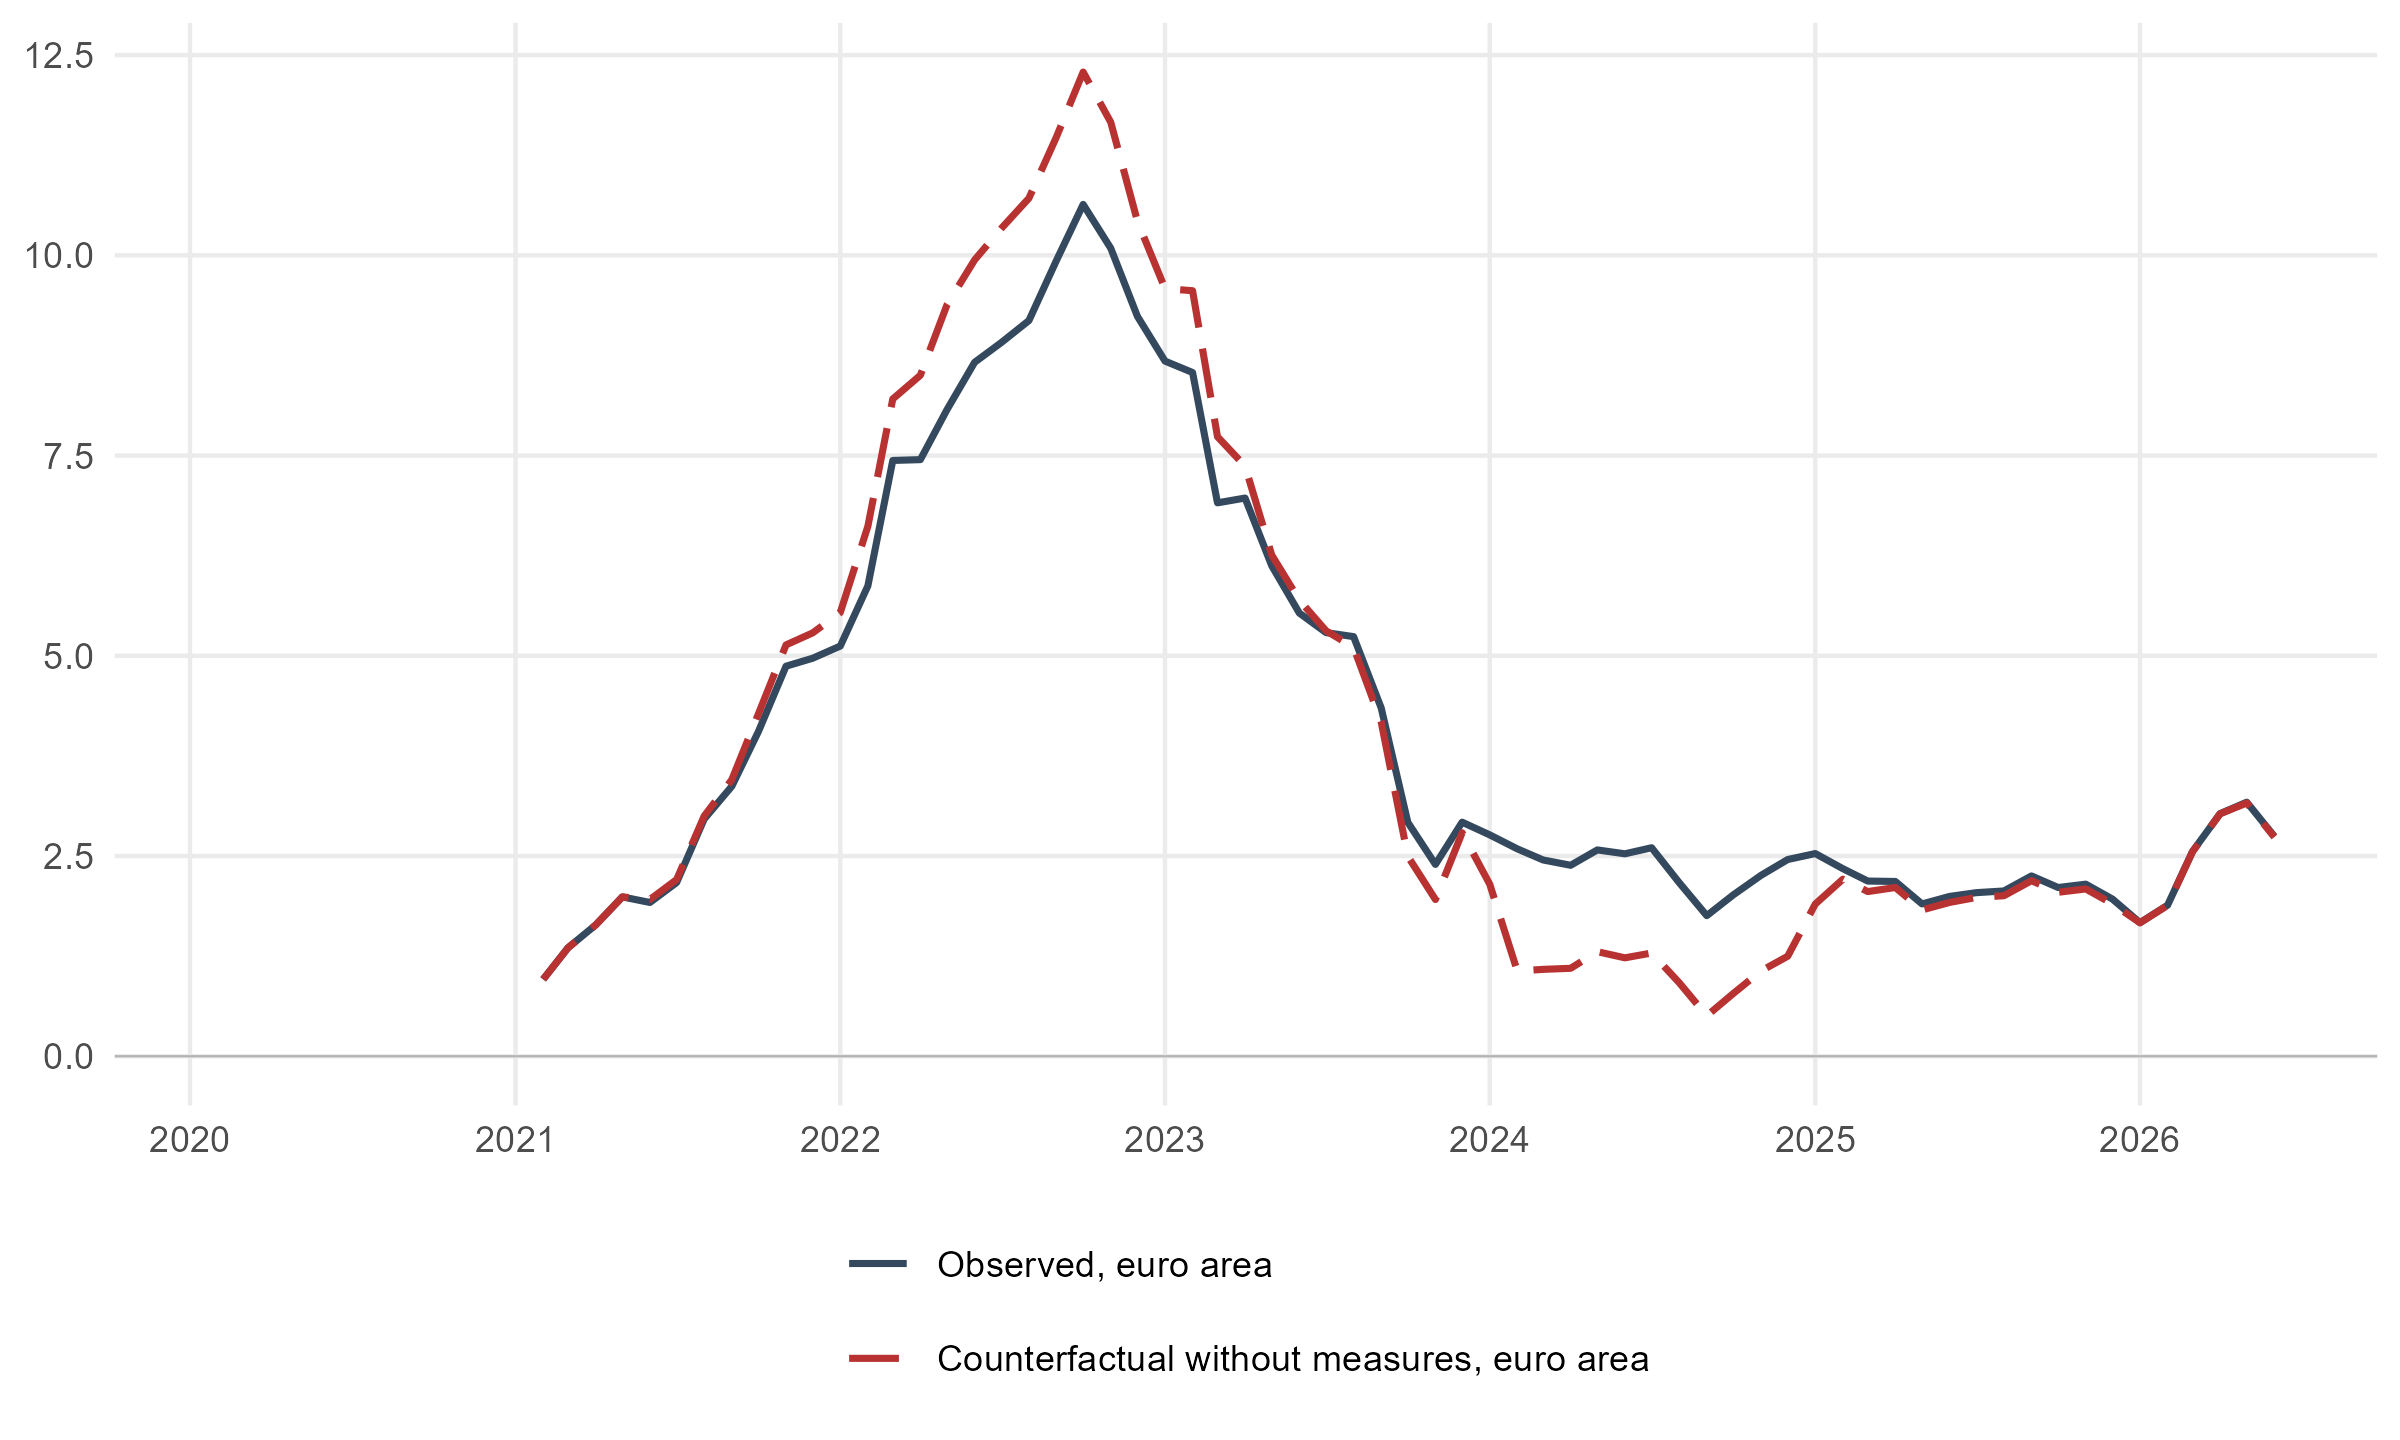
\includegraphics[width=.94\textwidth,height=.64\textheight,keepaspectratio]{fig/policy_total_cpi_counterfactual_inflation_EA_policy_sample.png}
\source{Eurostat HICP and HBS; authors\textquotesingle\ calculations.}
\end{frame}

% Slide 21; speaking time 1 min; cumulative 28.5 min.
% Evidence: main.tex, country policy table; existing derived annual gap graphic
\begin{frame}{Policy Effects on the Q1--Q5 Gap}
\noindent{\small\color{WarmGray}Price measures can narrow the Q1--Q5 gap without income targeting: electricity and gas support reduced the gap, while fuel support partly offset this effect in 2022.\par}
\vspace{0.3em}
\centering
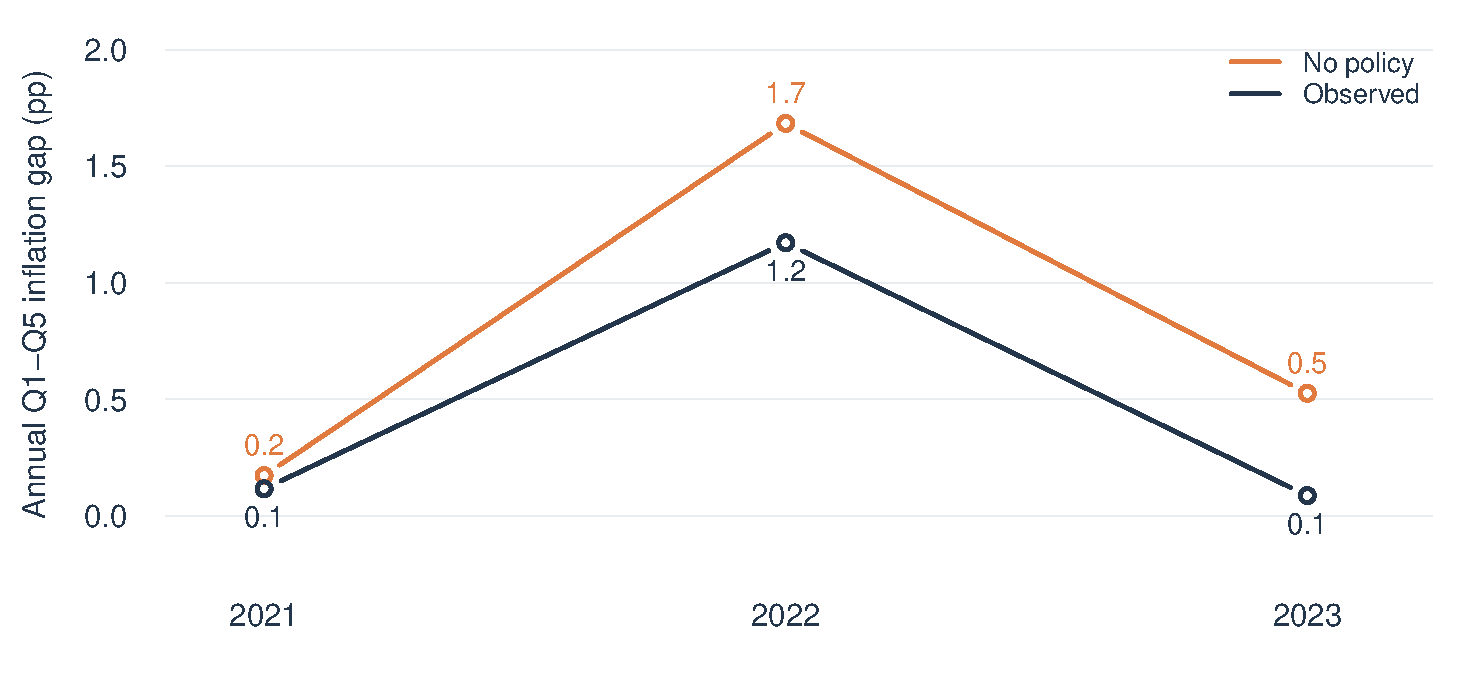
\includegraphics[width=0.98\textwidth,height=0.57\textheight,keepaspectratio]{fig/slide15_observed_no_policy_q1_q5_gap.pdf}
\source{Eurostat and national statistical institutes; authors' calculations. Annual-average Q1--Q5 inflation-rate gaps, in percentage points.}
\end{frame}

% Slide 22; speaking time 1.5 min; cumulative 30 min.
% Evidence: Promoted from appendix; main.tex product effects; fuels are a subset of vehicle operation
\begin{frame}{Household Energy Accounts for Most of the Gap Reduction}
\centering
\footnotesize
\begin{tabular}{lrrrrrr}
\toprule
& \multicolumn{3}{c}{Average-inflation effect} & \multicolumn{3}{c}{Q1--Q5 inequality effect}\\
\cmidrule(lr){2-4}\cmidrule(lr){5-7}
Product group & 2021 & 2022 & 2023 & 2021 & 2022 & 2023\\
\midrule
Food and non-alcoholic beverages & 0.0 & 0.0 & -0.1 & 0.0 & 0.0 & 0.0\\
Housing energy & -0.1 & -1.0 & -0.6 & -0.1 & -0.6 & -0.4\\
Vehicle operation & 0.0 & -0.3 & 0.3 & 0.0 & 0.1 & 0.0\\
All other products & 0.0 & 0.0 & 0.0 & 0.0 & 0.0 & 0.0\\
\midrule
\textbf{Total} & \textbf{-0.1} & \textbf{-1.4} & \textbf{-0.3} & \textbf{-0.1} & \textbf{-0.5} & \textbf{-0.4}\\
\bottomrule
\end{tabular}
\vspace{0.7em}
\begin{itemize}
  \item Household energy lowers the Q1--Q5 gap by \textbf{0.6 point in 2022} and \textbf{0.4 point in 2023}; the 2022 fuel effect offsets 0.1 point.
\end{itemize}
\source{Eurostat and national statistical institutes; authors' calculations. Product contributions to annual policy effects, in percentage points.}
\end{frame}

% Slide 23; speaking time 1 min; cumulative 31 min.
% Evidence: Promoted from appendix; main.tex country effects
\begin{frame}{Policy Effects Differed Sharply Across Countries and Years}
\noindent{\small A positive later inflation effect can coexist with lower prices while support was active.\par}\vspace{.5em}
\centering
\small
\setlength{\tabcolsep}{4pt}
\begin{tabular}{lrrrrrr}
\toprule
& \multicolumn{3}{c}{Average-inflation effect} & \multicolumn{3}{c}{Q1--Q5 inequality effect}\\
\cmidrule(lr){2-4}\cmidrule(lr){5-7}
Country & 2021 & 2022 & 2023 & 2021 & 2022 & 2023\\
\midrule
Germany & 0.0 & -0.5 & -0.8 & 0.0 & -0.2 & -0.8\\
France & -0.1 & -2.4 & -0.5 & 0.0 & -1.0 & -0.4\\
Italy & -0.2 & -1.4 & 0.7 & -0.1 & -0.2 & -0.1\\
Spain & -0.5 & -2.1 & -0.4 & -0.2 & -0.8 & -0.4\\
Netherlands & 0.0 & -1.8 & -0.7 & 0.0 & -0.7 & -0.7\\
Portugal & 0.0 & -0.9 & -1.5 & 0.0 & -0.3 & -0.9\\
Slovakia & 0.0 & 0.0 & -3.1 & 0.0 & 0.0 & -2.0\\
\midrule
\textbf{Euro area} & \textbf{-0.1} & \textbf{-1.4} & \textbf{-0.3} & \textbf{-0.1} & \textbf{-0.5} & \textbf{-0.4}\\
\bottomrule
\end{tabular}
\par\smallskip{\small Negative values indicate lower inflation or a smaller Q1--Q5 gap.\par}
\source{Eurostat and national statistical institutes; authors' calculations. Entries are observed minus no-policy annual-average inflation rates, in percentage points.}
\end{frame}

% Slide 24; speaking time 1.5 min; cumulative 33.5 min.
% Evidence: main.tex, household methodology
\begin{frame}{Household Microdata Reveal Individual Exposure}
\begin{itemize}
\setlength{\itemsep}{.8em}
\item \textbf{An index for each household:} combine 2020 HBS baskets with HICP prices, excluding actual and imputed rents.
\item \textbf{RAS calibration:} match household expenditure margins and annual HICP product shares.
\item \textbf{A consistent micro--macro link:} revalued-expenditure weights make mean household inflation equal to growth of the aggregate microdata index (Appendix A2).
\end{itemize}
\end{frame}

% Slide 25; speaking time 2.5 min; cumulative 36 min.
% Evidence: main.tex, household distribution figure, 2022 panel and common axis
\begin{frame}{Policies Shifted the Household Inflation Distribution in 2022}
\noindent{\small Shares of revalued expenditure; 19 euro-area countries (Portugal excluded).\par}
\centering
% Same RAS distribution output as main.tex: 2022 panel and common x-axis.
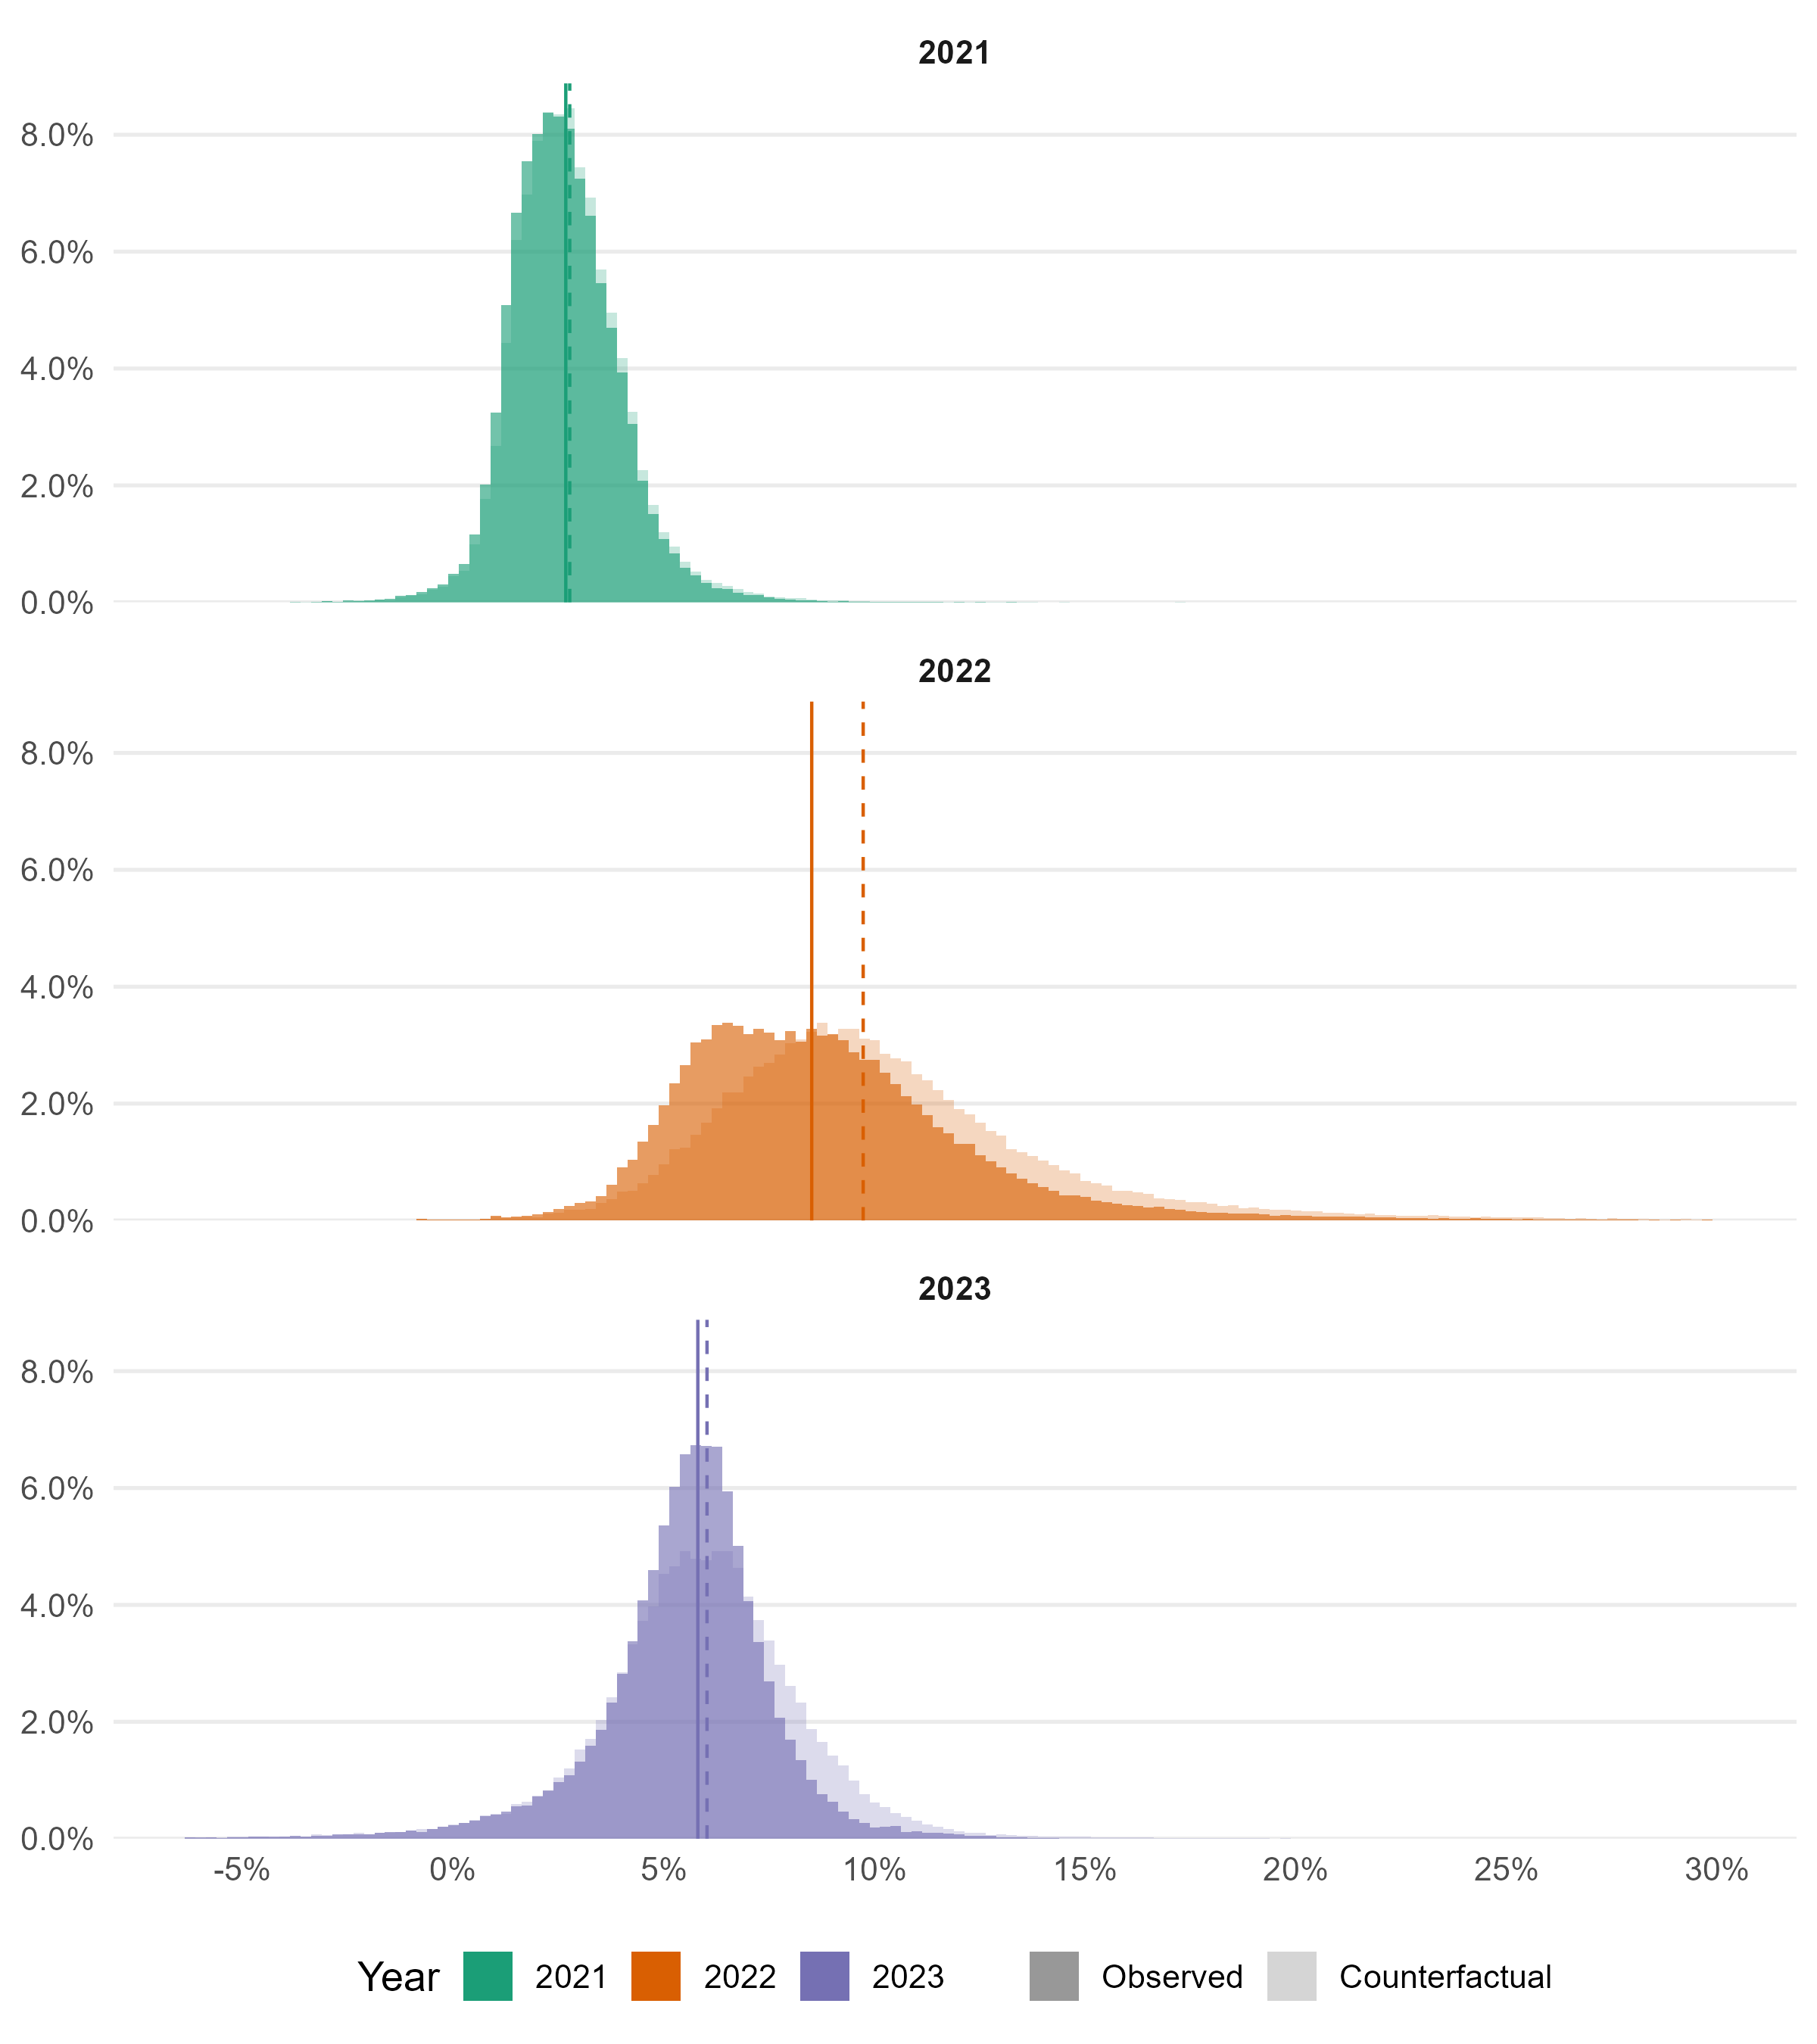
\includegraphics[width=.72\textwidth,trim=0 254bp 0 206bp,clip]{fig/fig_EA20_household_observed_counterfactual_distribution_2021_2023.png}
\par\vspace{-.4em}
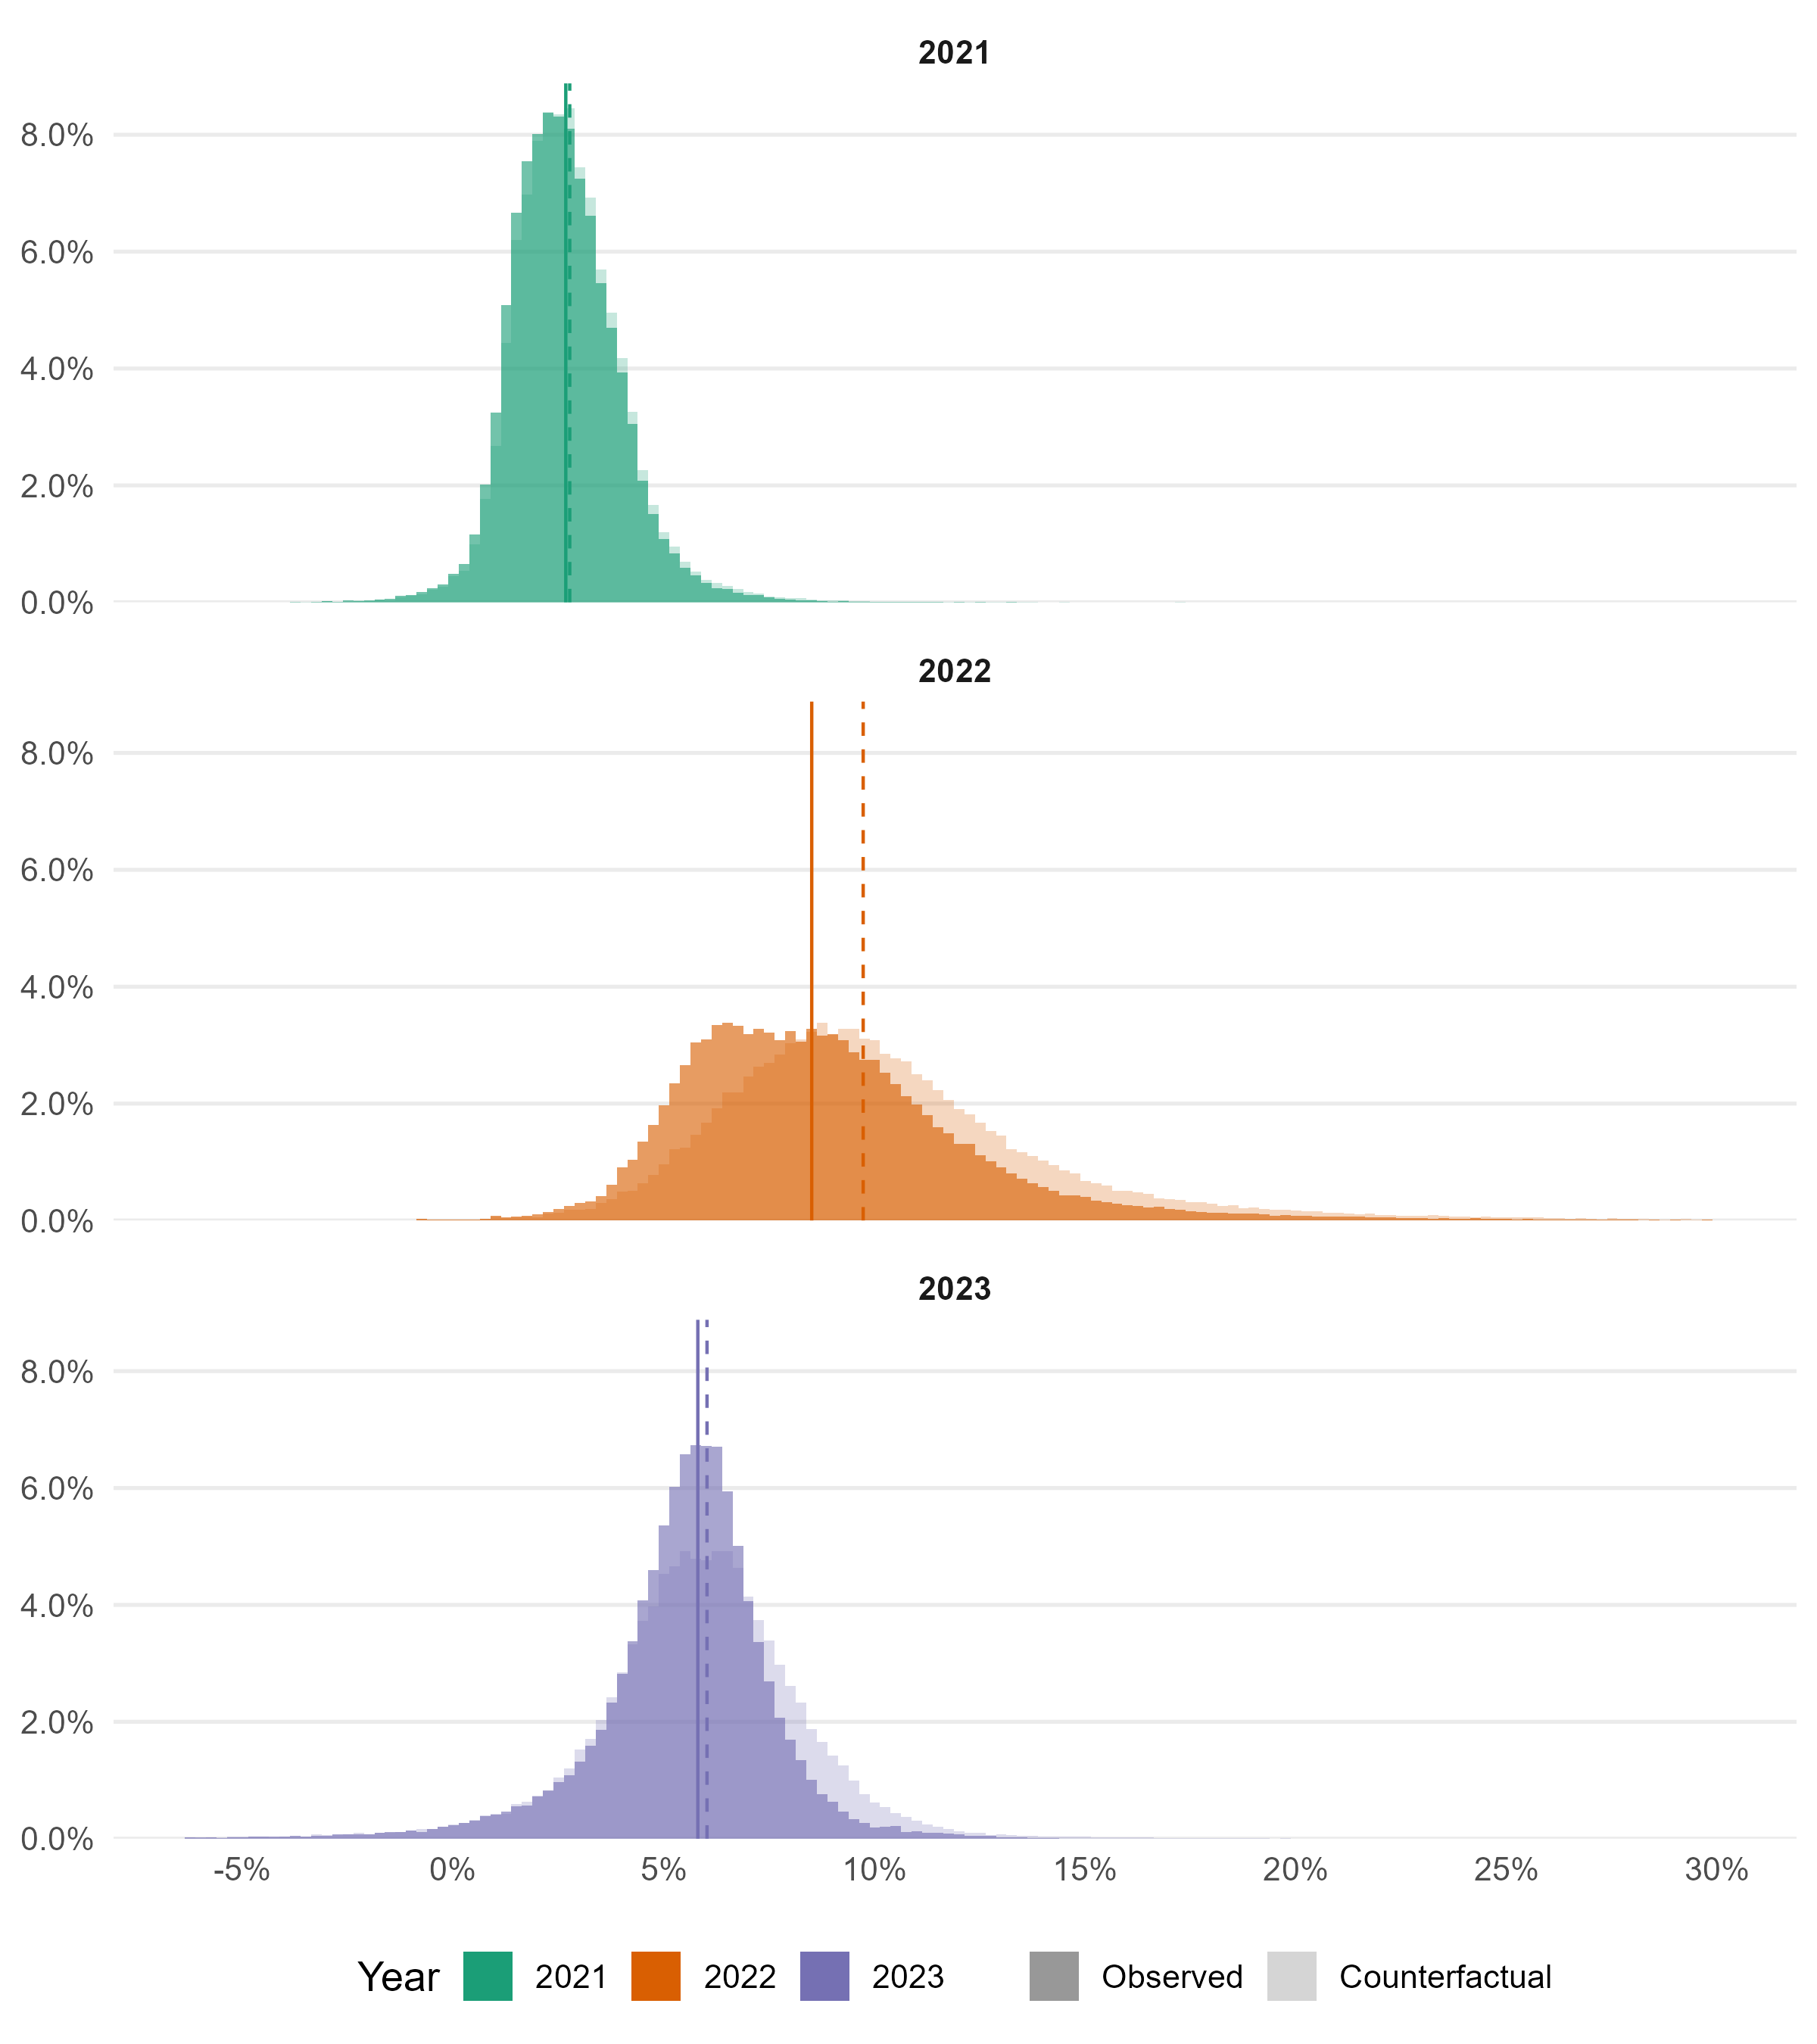
\includegraphics[width=.72\textwidth,trim=0 44bp 0 589bp,clip]{fig/fig_EA20_household_observed_counterfactual_distribution_2021_2023.png}
\par\smallskip
{\small Annual inflation (\%); darker/solid: observed; lighter/dashed: no policy.\par}
\vspace{.2em}\raggedright
{\small\textbf{Revalued-expenditure-weighted medians:} observed \textbf{8.5\%}; no policy \textbf{9.7\%}.\par}
\vspace{.3em}
{\small Difference between scenario medians: \textbf{1.2 pp}, not the median household policy effect.\par}
\source{Eurostat HICP and 2020 HBS; authors' calculations. RAS, COICOP digit 3, rents excluded; same baskets and HICP margins in both scenarios.}
\end{frame}

% Slide 26; speaking time 1.5 min; cumulative 37.5 min.
% Evidence: main.tex, household dispersion table; replaces legacy French variance as headline evidence
\begin{frame}{Substantial Dispersion Remains Within Countries}
\noindent{\small Unweighted ANOVA; 138,797 households per year in 17 countries.\par}
\vspace{.4em}\centering\small\renewcommand{\arraystretch}{1.2}
\begin{tabular}{lrrr}
\toprule
Share of variance (\%) & 2021 & 2022 & 2023\\
\midrule
\multicolumn{4}{l}{\textit{Partition of total variance}}\\
Between countries & 34.61 & 55.69 & 59.61\\
Within countries & 65.39 & 44.31 & 40.39\\
\midrule
\multicolumn{4}{l}{\textit{Partition of within-country variance}}\\
Household characteristics & 2.80 & 6.63 & 1.17\\
Residual & 97.20 & 93.37 & 98.83\\
\bottomrule
\end{tabular}
\par\vspace{.6em}\raggedright
{\small In 2022, household characteristics explain \textbf{6.63\% of within-country variance}; \textbf{93.37\%} remains unexplained.\par}
\source{Main paper, household-inflation ANOVA. RAS, COICOP digit 3, rents excluded. Country effects enter first, then income quintile, age, household size, education and residence. Each panel has its own denominator; contributions are descriptive.}
\end{frame}

% Slide 27; speaking time 1.5 min; cumulative 39 min.
% Evidence: main.tex, annual household regression table
\begin{frame}{Income, Age and Residence Gradients Peaked in 2022}
\noindent{\small Unweighted OLS; 138,797 households per year in 17 countries.\par}
\vspace{.5em}\centering\small\renewcommand{\arraystretch}{1.25}
\begin{tabular}{lrrr}
\toprule
Conditional inflation difference (pp) & 2021 & 2022 & 2023\\
\midrule
Q5 relative to Q1 & 0.05 & -1.29$^{***}$ & -0.35\\
 & (0.15) & (0.27) & (0.29)\\
Under 30 relative to 60+ & -0.01 & -1.25$^{***}$ & -0.51$^{***}$\\
 & (0.09) & (0.20) & (0.14)\\
Cities relative to rural areas & -0.47$^{***}$ & -1.08$^{***}$ & 0.30$^{***}$\\
 & (0.09) & (0.12) & (0.10)\\
\bottomrule
\end{tabular}
\par\vspace{.6em}\raggedright
{\small Controls: income quintile, age, household size, education, residence and country fixed effects. Conditional associations, not causal effects.\par}
\source{Main paper, household-inflation regressions. RAS, COICOP digit 3, rents excluded. Country-clustered standard errors in parentheses; $^{***}p<0.01$. Italy, Portugal and the Netherlands excluded.}
\end{frame}



% Slide 28; speaking time 1.5 min; cumulative 40.5 min.
% Evidence: Promoted from appendix; main.tex, inflation burden
\begin{frame}{Inflation Burden Is Larger for Low-Income Households}
\centering
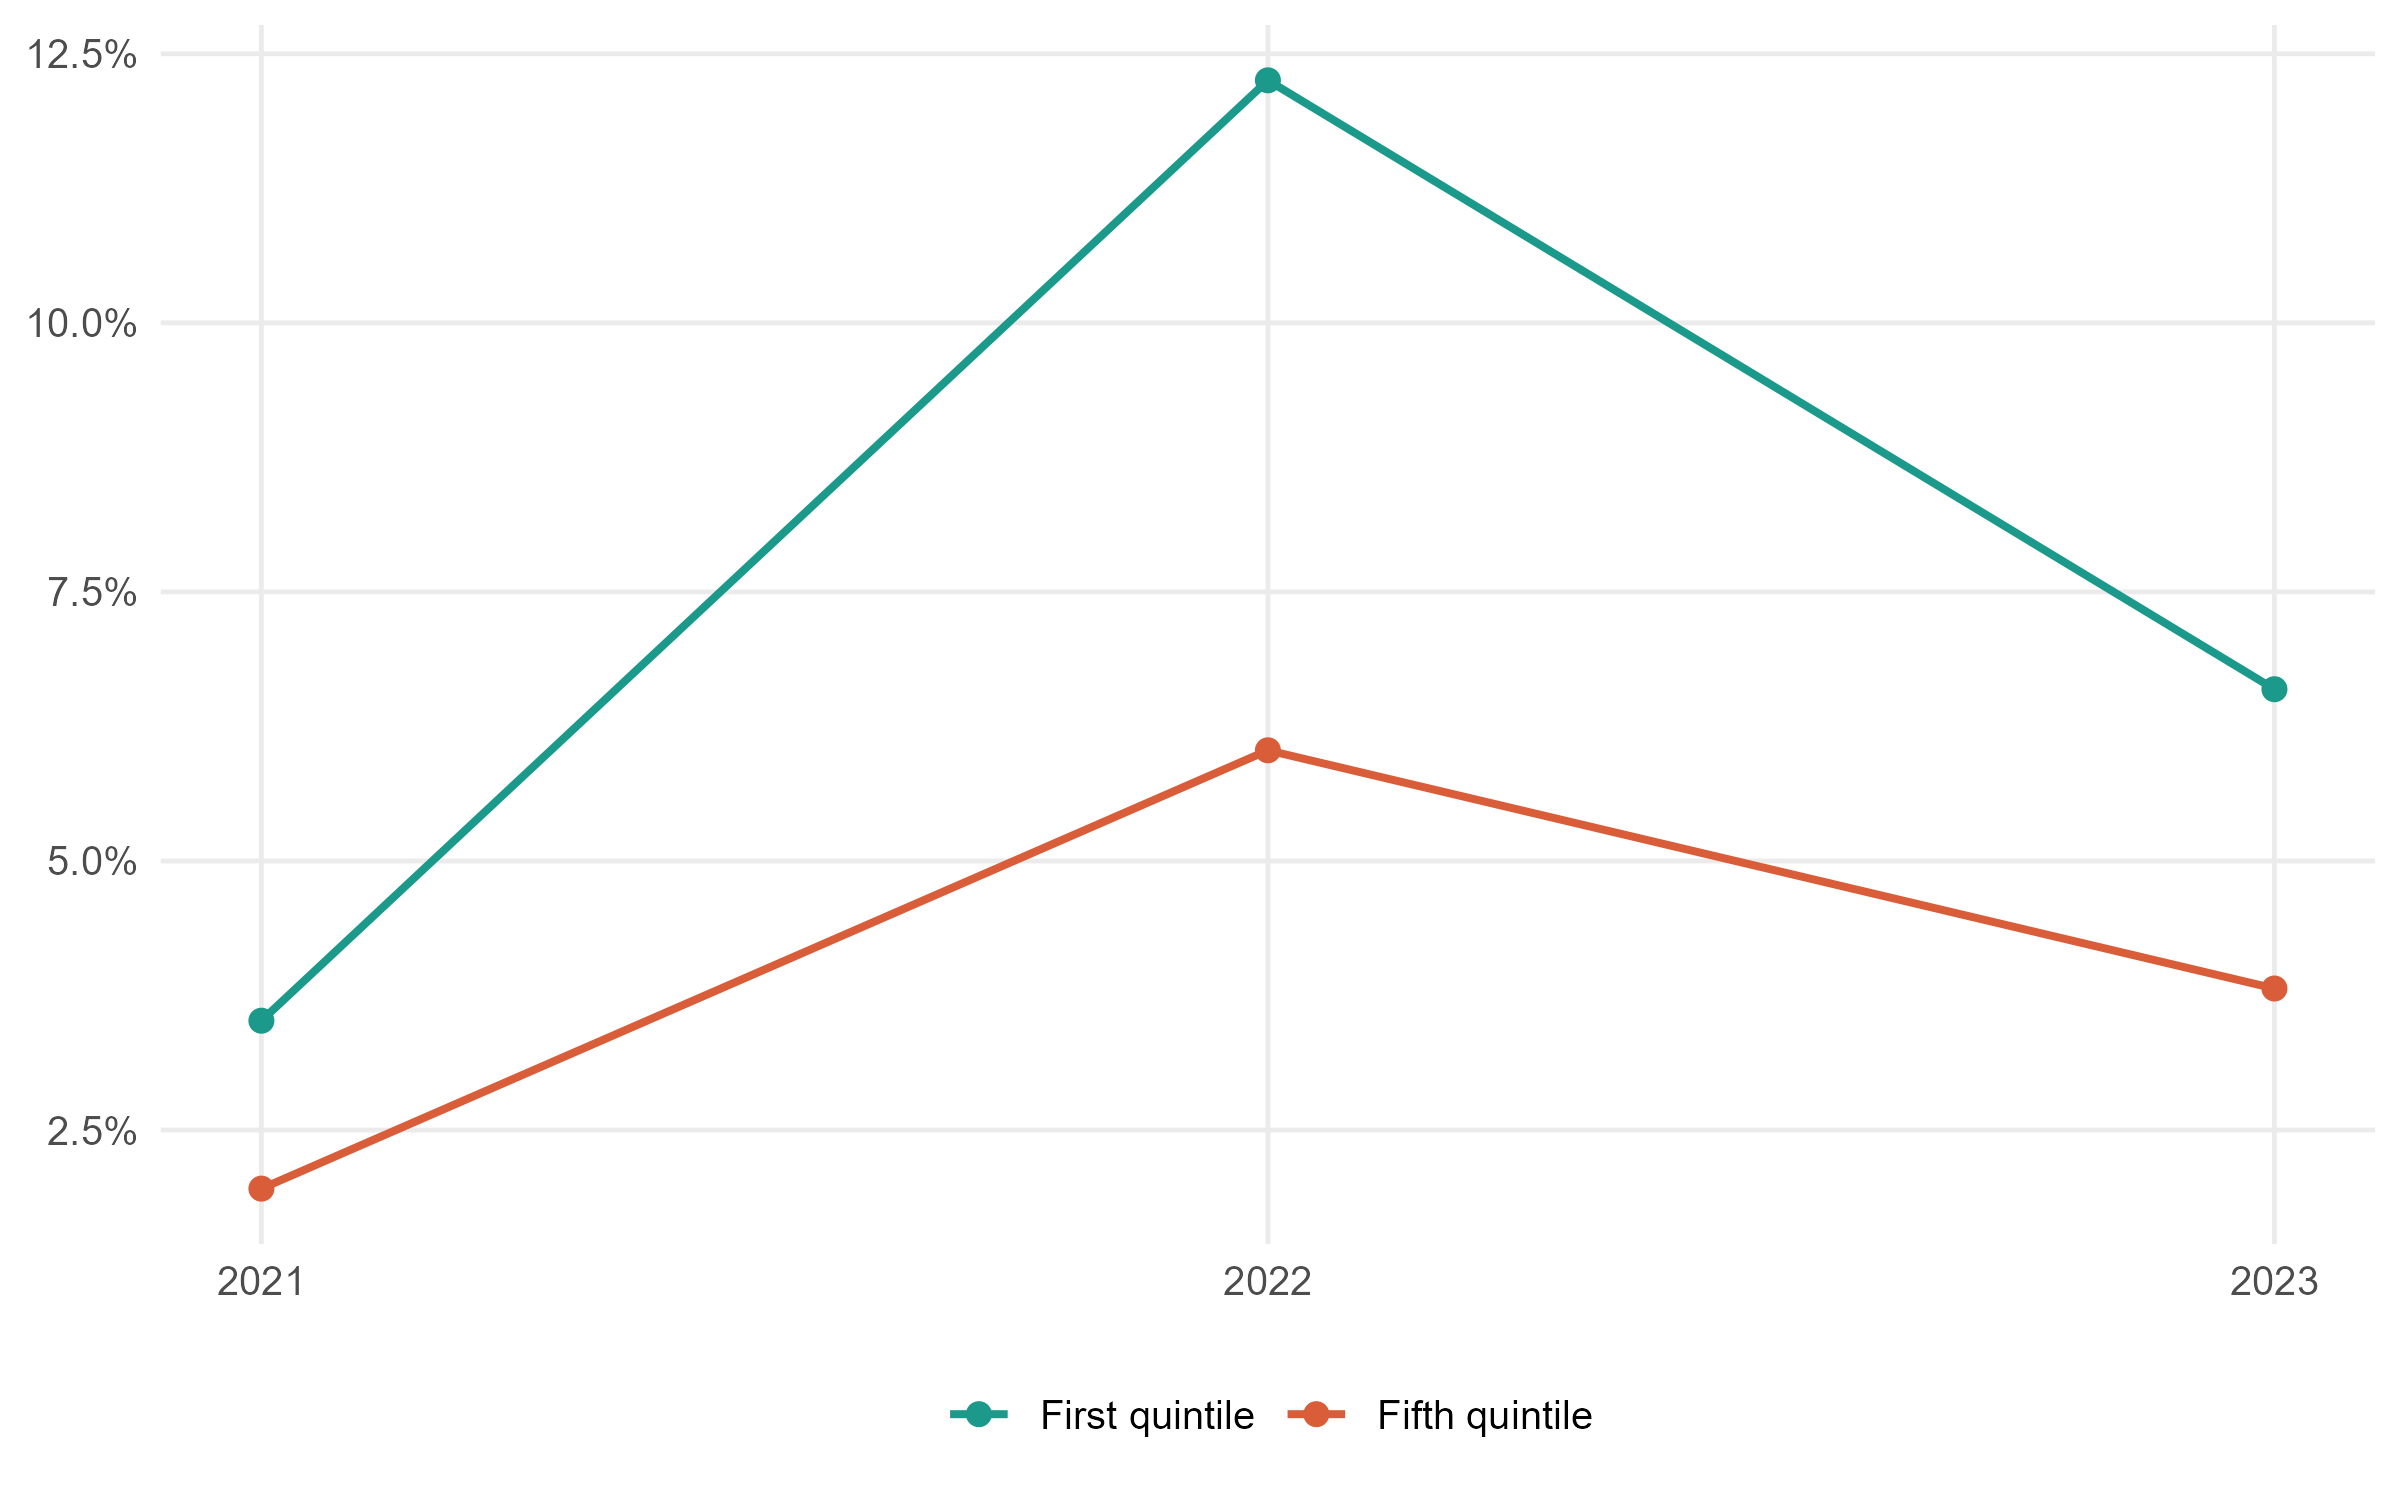
\includegraphics[width=0.70\textwidth,height=0.53\textheight,keepaspectratio]{fig/fig_EA20_2019_2026_income_inflation_burden_Q1_Q5.png}
\begin{itemize}
  \item The Q1 burden reached \textbf{3.5\%, 12.3\%, and 6.6\%} of net income in 2021--2023, versus \textbf{2.0\%, 6.1\%, and 3.8\%} for Q5.
\end{itemize}
\par\smallskip{\small Scaled price exposure using 2020 resources, not an observed loss of real income or welfare.\par}
\source{Eurostat HICP and HBS microdata; authors' calculations. 18-country sample; scaled non-rent exposure, in percent of net income. Ratios winsorized at the national 99th percentile.}
\end{frame}

% Slide 29: conclusion of the main presentation.
% Evidence: slides 2, 4, 11--16, 25--28 and 30--33; framing informed by IBFI 2025.
\begin{frame}{Conclusion}
\begin{itemize}
\setlength{\itemsep}{.8em}
\item \textbf{Comparable measures across countries.} HICP prices and household budgets provide monthly inflation indices by income, age and residence.
\item \textbf{Unequal exposure to the inflation surge.} Energy and food hit low-income households harder, with large differences across countries and a larger burden relative to income.
\item \textbf{Price policies cushioned the shock.} In 2022, they lowered inflation by 1.4 percentage points and the Q1--Q5 gap by 0.5 point, mainly through electricity and gas support.
\item \textbf{Group averages conceal substantial dispersion.} Household-level data are essential; assessing the full distributional impact also requires income and wealth.
\end{itemize}
\end{frame}

\appendix
\setcounter{framenumber}{0}
\setbeamertemplate{footline}{\hfill\raisebox{.6em}{\scriptsize\color{WarmGray}Appendix \insertframenumber/19}\hspace{1em}}

% Unnumbered white divider, following the conclusion.
\begin{frame}[plain,noframenumbering]
  \centering
  \vfill
  {\Huge Appendix\par}
  \vfill
\end{frame}

% Appendix block: Methods and coverage

% Appendix 1: Group and Household Indices Both Exclude Rents
\begin{frame}{Group and Household Indices Both Exclude Rents}
\begin{itemize}
\item Exclude actual and imputed rents (HBS 041 and 042) and corresponding HICP rent components before matching and aggregation.
\item Reconstruct parent housing categories without rents and normalize weights over matched non-rent products.
\item Both group and household indices use RAS calibration to annual HICP product margins, with matched non-rent coverage.
\end{itemize}
\par\vspace{.5em}
Rent sensitivity and official all-items validation retain their explicitly stated reference coverage.
\source{Main paper, Data and Methodology; RAS Weighting appendix.}
\end{frame}

% Appendix 2: RAS Calibration and the Micro--Macro Link
\begin{frame}{RAS Calibration and the Micro--Macro Link}
\small
\setlength{\abovedisplayskip}{4pt}\setlength{\belowdisplayskip}{4pt}\setlength{\abovedisplayshortskip}{3pt}\setlength{\belowdisplayshortskip}{3pt}
$a_{ic}$: survey weight; $E_{ic}$: non-rent expenditure; $\bar I_{ic,y}$: annual-average price index.
\par\vspace{.4em}
\textbf{RAS calibration:} household margins and annual HICP product shares.
\[
s_{ic}=\frac{a_{ic}E_{ic}}{\sum_h a_{hc}E_{hc}},\qquad
\sum_j M_{j,ic,y}=s_{ic},\qquad
\sum_i M_{j,ic,y}=\omega^{\mathrm{HICP}}_{j,c,y},\qquad
\omega_{j,ic,y}=\frac{M_{j,ic,y}}{s_{ic}}.
\]
\textbf{Aggregation identity on the same microdata:}
\[
\lambda_{ic,y}=\frac{a_{ic}E_{ic}\bar I_{ic,y-1}}
{\sum_h a_{hc}E_{hc}\bar I_{hc,y-1}},\qquad
\bar\pi_{ic,y}=100\left(\frac{\bar I_{ic,y}}{\bar I_{ic,y-1}}-1\right).
\]
\[
\underbrace{\sum_i\lambda_{ic,y}\bar\pi_{ic,y}}_{\text{Weighted mean household inflation}}
=\underbrace{100\left(\frac{\sum_i a_{ic}E_{ic}\bar I_{ic,y}}
{\sum_i a_{ic}E_{ic}\bar I_{ic,y-1}}-1\right)}_{\text{Growth of the aggregate microdata index}}.
\]
\textbf{Check by country-year:} same households and baskets; difference $=0$ up to numerical precision.
\source{Main paper, Calculating Household Inflation Rates. Algebraic identity; numerical check not reported here. Agreement with published HICP additionally requires consistent prices, coverage and expenditure profiles.}
\end{frame}

% Appendix 3: Inflation Burden Scales Exposure by Household Resources
% Moved from main presentation to appendix.
% Evidence: main.tex, burden definition and coverage
\begin{frame}{Inflation Burden Scales Exposure by Household Resources}
For household $i$ in country $c$, the raw exposure measure is
\[
\mathcal B^{\mathrm{raw}}_{ic,y}=\bar\pi_{ic,y}\frac{X_{ic}}{Y_{ic}}.
\]
\begin{itemize}
\item $\bar\pi$: annual household inflation (\%); $X$: total expenditure; $Y$: net income, both from the 2020 HBS.
\item Winsorize expenditure-to-income ratios at the national survey-weighted 99th percentile, then aggregate household burdens.
\item Non-rent inflation is scaled by total expenditure: this measures exposure relative to income, rather than an exact welfare loss.
\end{itemize}
\source{Main paper, Inflation Burden. 18-country sample; Italy and Portugal excluded.}
\end{frame}

% Appendix 4: Reconstructing Prices Without the Measures
% Evidence: main.tex, counterfactual construction
\begin{frame}{Reconstructing Prices Without the Measures}
For each affected product $j$ and month $t$, replace its observed price index:
\[
\widetilde P_{j,t}=P_{j,t}\frac{\widetilde p_{j,t}}{p_{j,t}}.
\]
\begin{itemize}
\item Use statutory tax rates, unit rebates or documented reference tariffs when available.
\item Calibrate an aggregate-equivalent price wedge when monthly tariffs, coverage or unit prices are unavailable.
\item Retain observed prices for unaffected products and apply the same household weights and index construction.
\end{itemize}
\end{frame}

% Appendix block: Validation and aggregation

% Appendix 5: All-Items Reference: RAS Tracks the Published HICP
% Moved from main presentation to appendix.
% Evidence: Promoted from appendix; main.tex validation figure
\begin{frame}{All-Items Reference: RAS Tracks the Published HICP}
\centering
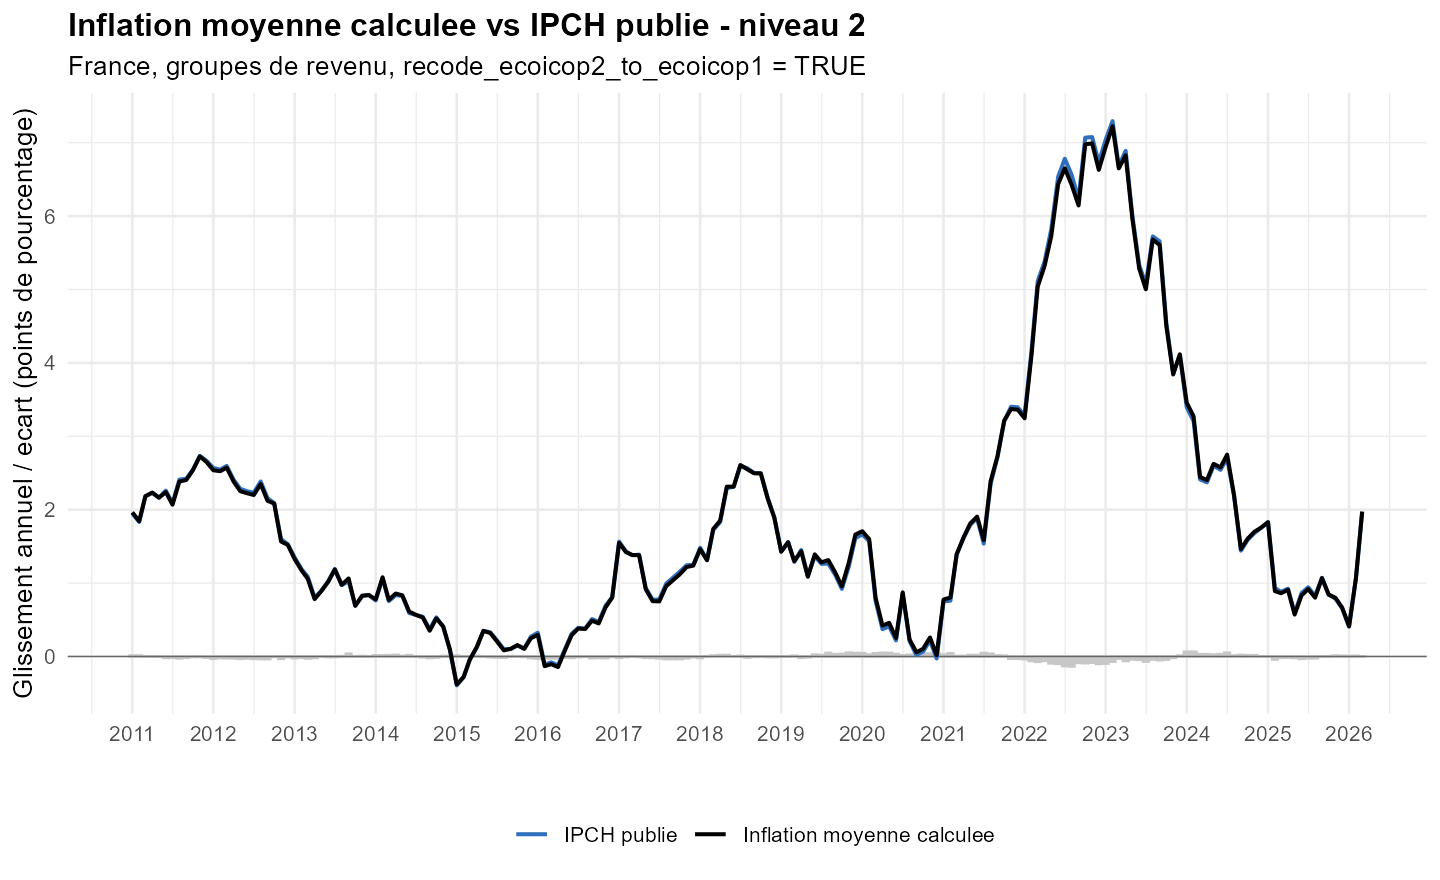
\includegraphics[width=0.96\textwidth,height=0.72\textheight,keepaspectratio]{fig/fig_FR_2010_2026_hicp_inflation_validation_level2_recode_mean_vs_published.png}
\source{INSEE, Eurostat; authors' calculations. Original all-items validation; not the excluding-rents baseline. Year-on-year inflation (\%).}
\end{frame}

% Appendix 6: Finer Product Detail Can Widen or Narrow Income Gaps
% Evidence: main.tex, aggregation bias appendix and its table
\begin{frame}{Finer Product Detail Can Widen or Narrow Income Gaps}
\centering\small\renewcommand{\arraystretch}{1.3}
\begin{tabular}{lrrrrr}
\toprule
2022 Q1--Q5 gap (pp) & Macro D3 & Micro D2 & Micro D3 & Micro D4 & Micro D5\\
\midrule
Germany & 1.4 & 2.0 & 1.5 & -- & --\\
France & 0.2 & 0.3 & 0.3 & -- & --\\
Spain & 1.0 & 0.8 & 1.0 & -- & --\\
Netherlands & 2.8 & 2.0 & 3.0 & 2.5 & 1.9\\
Belgium & 2.3 & 2.5 & 2.3 & 2.4 & 2.3\\
Lithuania & 3.4 & 2.9 & 3.7 & 4.9 & 4.9\\
\bottomrule
\end{tabular}
\par\vspace{.7em}\raggedright
Finer detail can widen or narrow gaps. Dutch matched coverage: 99.3\% for macro D3, 99.9\% for micro D3, and 87.8\% for micro D5.
\source{Main paper, Aggregation Bias appendix. Selected countries; 18-country table in the paper. Macro: published HBS; micro: reconstructed total-income quintiles. RAS weights, rents excluded. Dashes: unavailable detail.}
\end{frame}

% Appendix block: Additional results

% Appendix 7: Inflation Inequality Was Highly Uneven Across Countries
\begin{frame}{Inflation Inequality Was Highly Uneven Across Countries}
\centering
\small
\renewcommand{\arraystretch}{1.0}
\setlength{\tabcolsep}{4pt}
\begin{tabular}{lrrr@{\qquad}lrrr}
\toprule
Country & 2021 & 2022 & 2023 & Country & 2021 & 2022 & 2023\\
\midrule
Austria & -0.5 & 0.1 & 0.5 & Ireland & 0.5 & 3.0 & 1.1\\
Belgium & 1.3 & 2.3 & -2.6 & Italy & 0.1 & 1.6 & 0.5\\
Croatia & 0.1 & 0.4 & -0.3 & Latvia & -0.2 & 4.8 & 2.5\\
Cyprus & 0.0 & 0.8 & 0.2 & Lithuania & 0.2 & 3.4 & 0.4\\
Estonia & 0.5 & 4.4 & 1.3 & Luxembourg & 0.1 & 0.2 & -0.1\\
Finland & -0.2 & -0.9 & 0.4 & Malta & -0.2 & 0.3 & 0.5\\
France & 0.3 & 0.2 & 0.2 & Netherlands & -0.2 & 2.8 & -0.9\\
Germany & -0.4 & 1.4 & 0.6 & Portugal & 0.8 & 0.2 & -0.9\\
Greece & 0.4 & 1.4 & -0.6 & Slovakia & -0.9 & 1.2 & 1.4\\
Spain & 0.8 & 1.0 & -0.7 & Slovenia & 0.1 & 0.5 & 1.4\\
\midrule
\multicolumn{4}{l}{\textbf{Euro area}} & & \textbf{0.1} & \textbf{1.2} & \textbf{0.1}\\
\bottomrule
\end{tabular}
\source{Eurostat HICP and HBS; authors' calculations. Units: Q1 minus Q5 annual-average inflation rates, in percentage points.}
\end{frame}

% Appendix 8: Older Households Faced Higher Inflation
% Evidence: main.tex, age figure
\begin{frame}{Older Households Faced Higher Inflation}
\centering
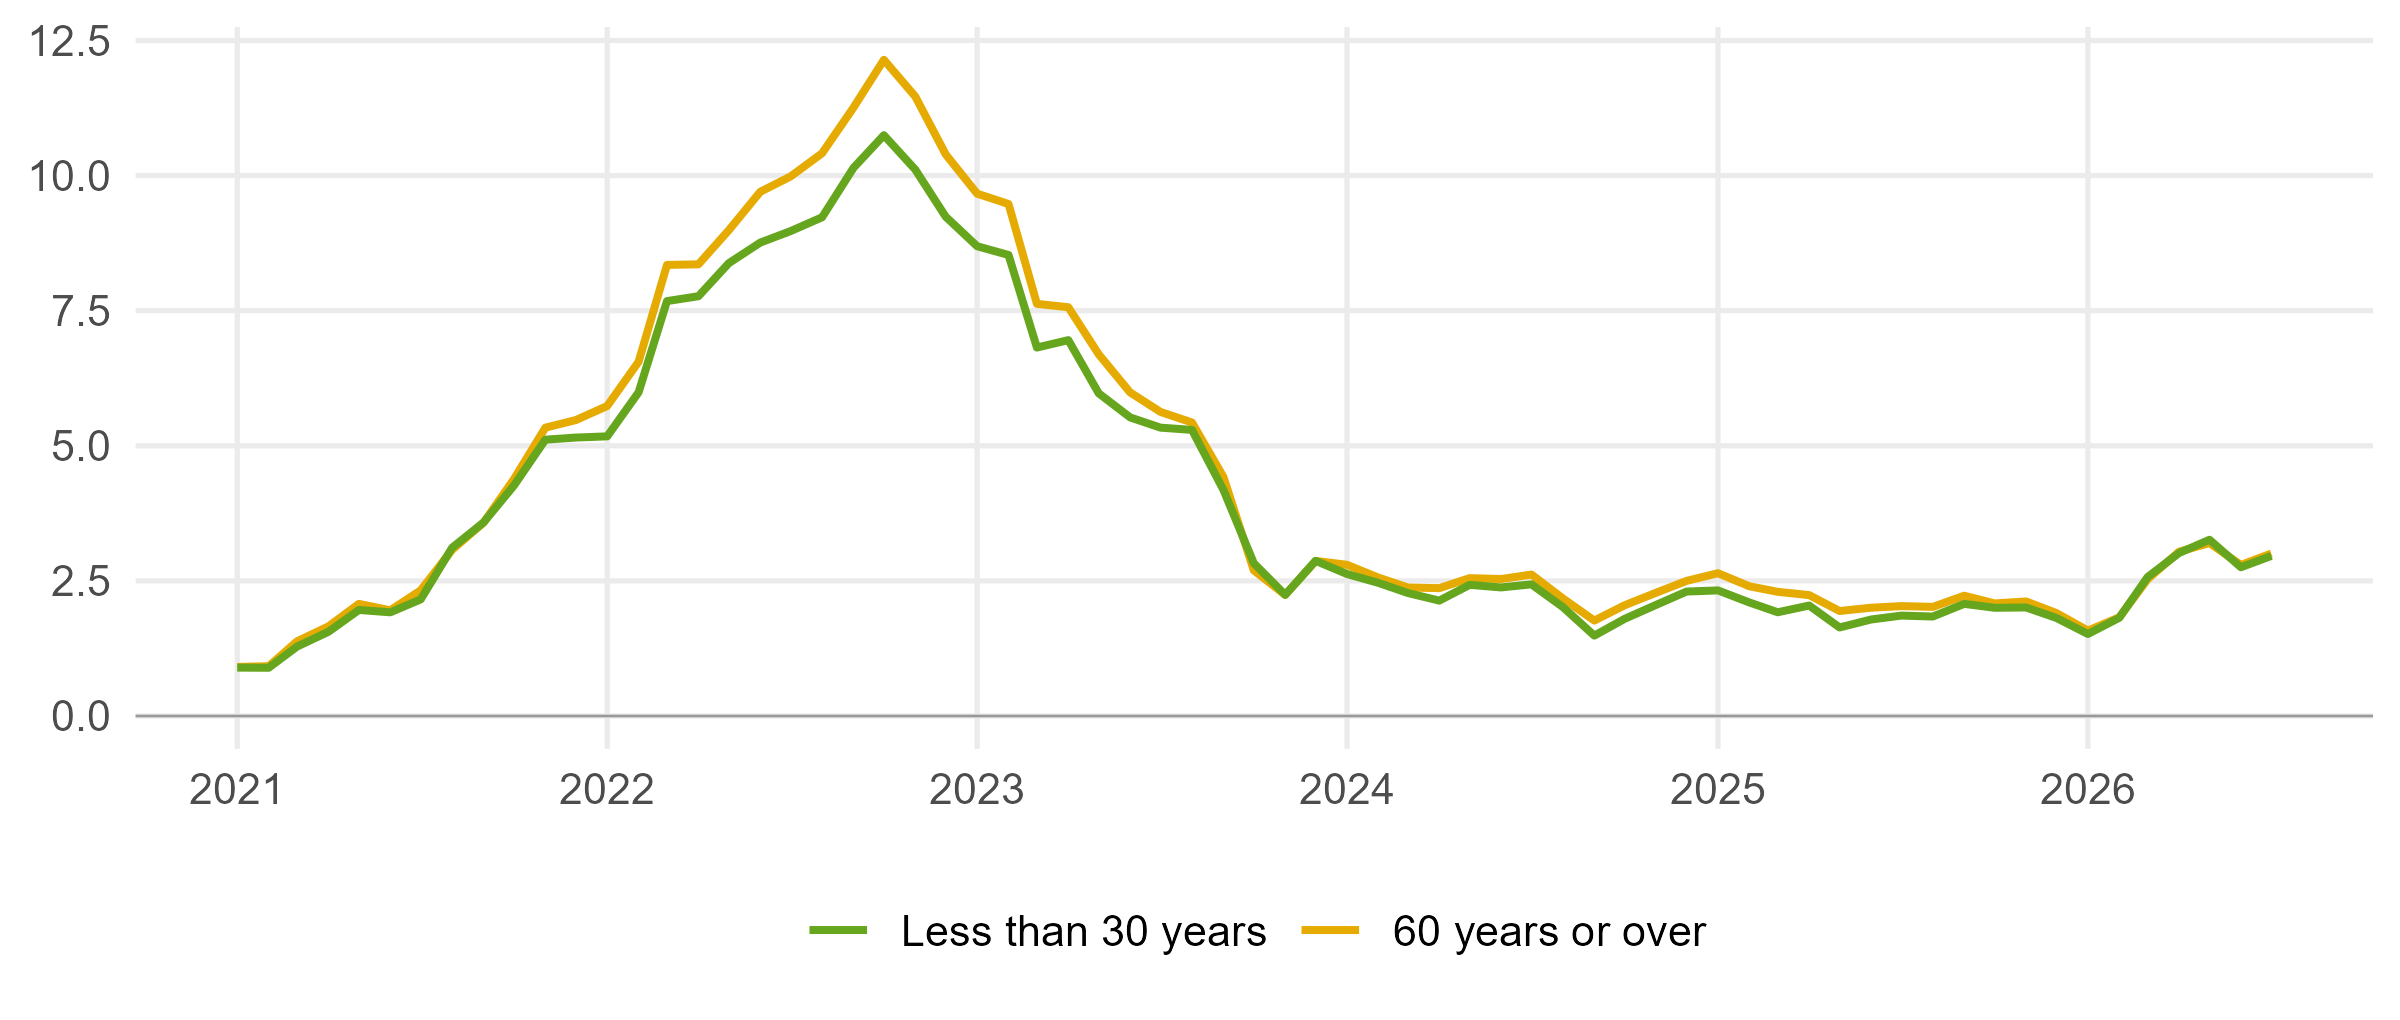
\includegraphics[width=0.82\textwidth,height=0.70\textheight,keepaspectratio]{fig/fig_EA20_2020_2026_age_inflation_under30_60plus.png}
\source{Eurostat HICP and HBS; authors' calculations. Units: year-on-year inflation, in percent.}
\end{frame}

% Appendix 9: Rural Households Faced Higher Inflation at the Peak
% Evidence: Promoted from appendix; main.tex residence figure
\begin{frame}{Rural Households Faced Higher Inflation at the Peak}
\centering
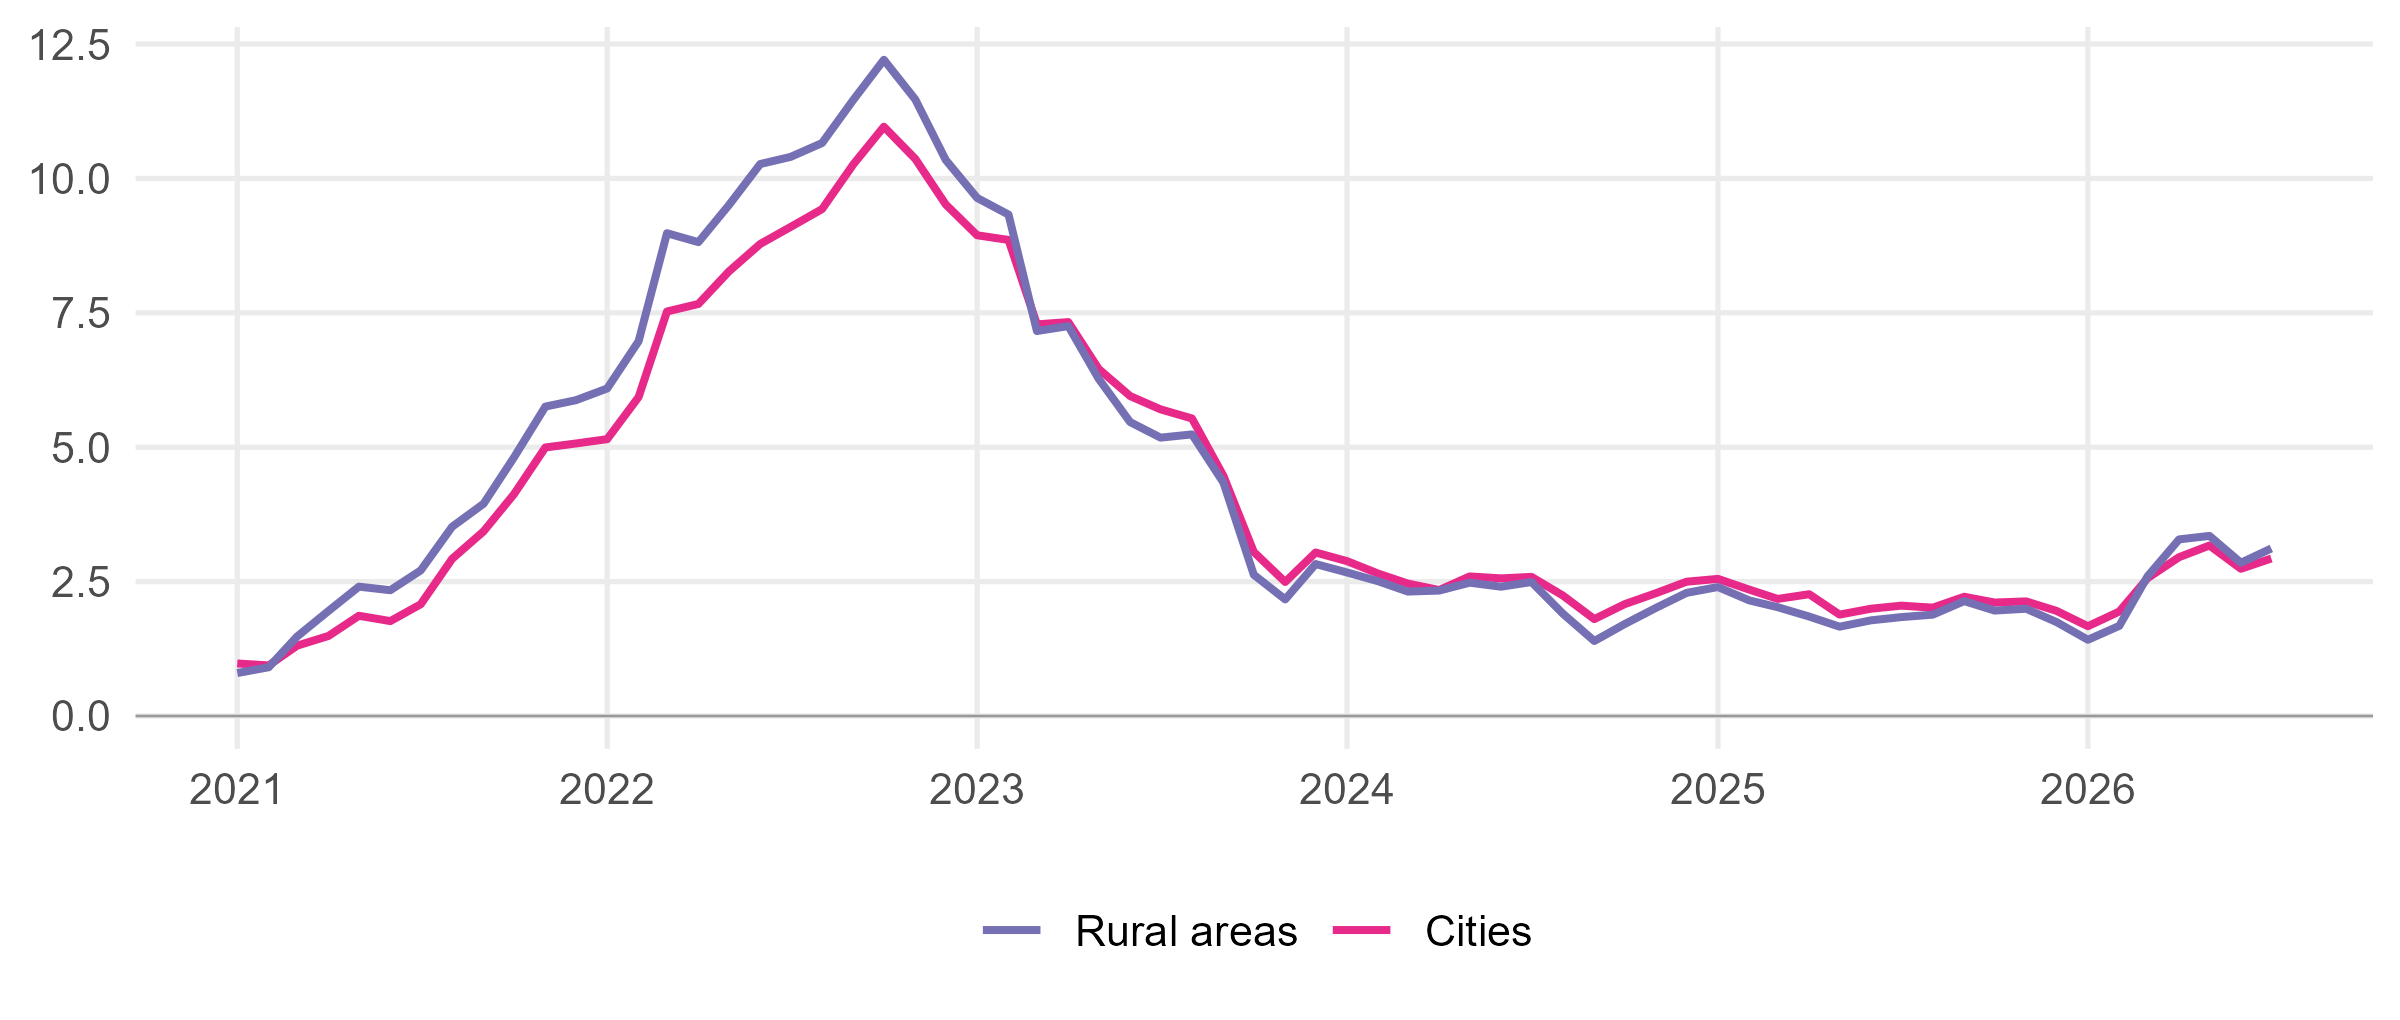
\includegraphics[width=0.78\textwidth,height=0.62\textheight,keepaspectratio]{fig/fig_EA20_2020_2026_urban_inflation_rural_cities.png}
\source{Eurostat HICP and HBS; authors' calculations. Units: year-on-year inflation, in percent.}
\end{frame}

% Appendix 10: Euro Area and US: Long-Run Inflation by Income
% US source supplied by user: Jaravel (2024); common end date May 2026.
\begin{frame}{Euro Area and US: Long-Run Inflation by Income}
\centering
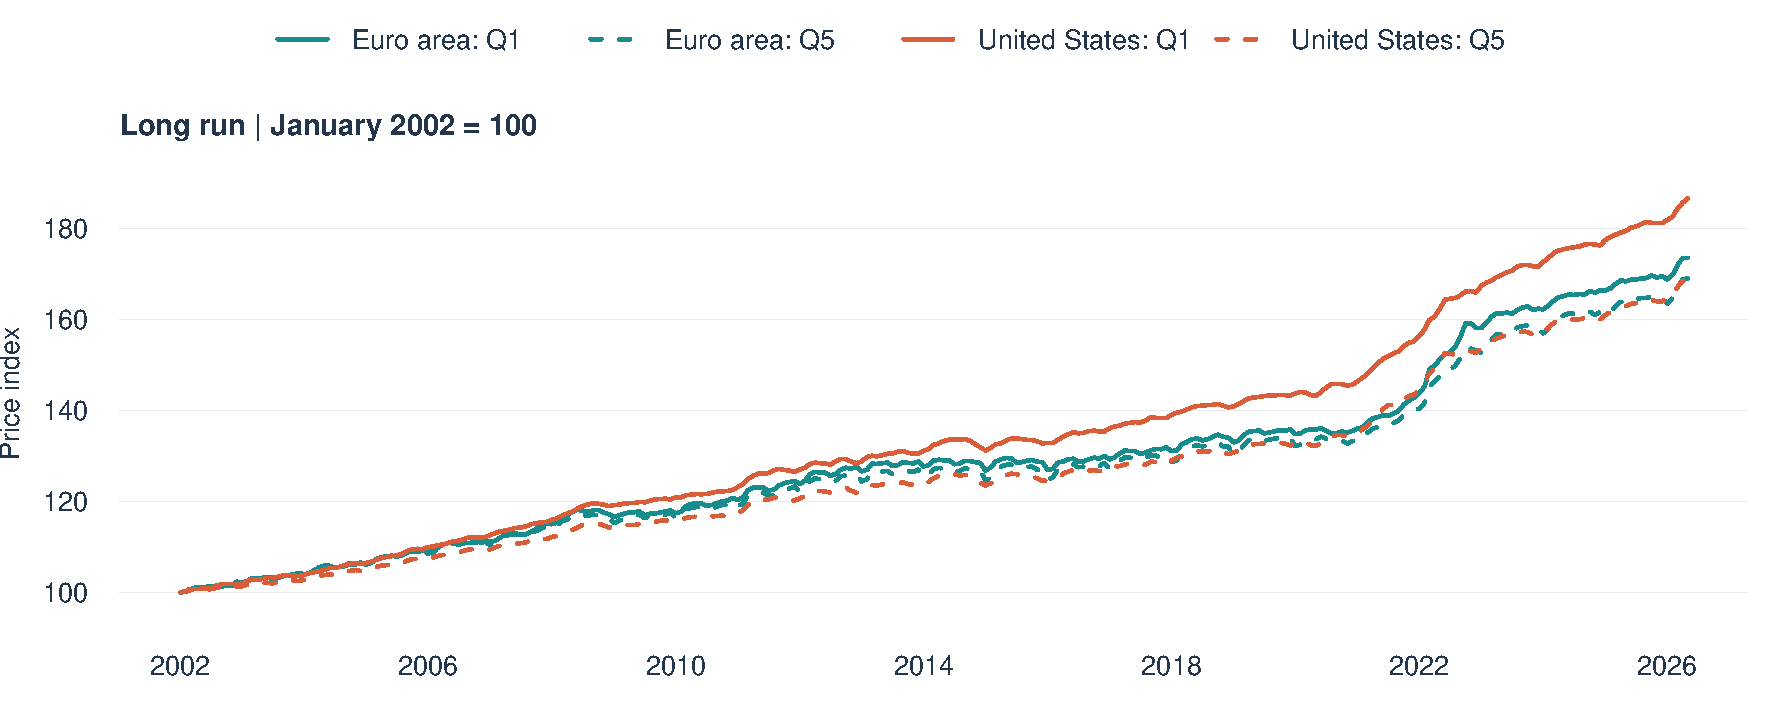
\includegraphics[width=\textwidth,height=.60\textheight,keepaspectratio]{fig/ea_us_income_comparison.pdf}
\par\smallskip\raggedright\small
By May 2026, cumulative Q1--Q5 gaps since 2002: \textbf{4.5 pp} (EA), \textbf{17.3 pp} (US).
\source{Euro area: HICP--HBS excluding rents. US: Jaravel (2024)}
\end{frame}

% Appendix 11: Direct and Indirect Exposure to Import-Price Shocks
\begin{frame}{Direct and Indirect Exposure to Import-Price Shocks}
\small
The observed 2022 extra-EU import-price increases are 83.9\% for energy and 21.0\% for food.
\[
\Delta\mathbf p^k=(\mathbf I-\mathbf A^{\mathsf T})^{-1}\mathbf b^k,
\qquad
\Delta\pi_g^k=\mathbf w_g^{\mathsf T}\mathbf C\mathbf d^k
+\mathbf w_g^{\mathsf T}\mathbf C\Delta\mathbf p^k.
\]
\begin{itemize}
\item $\mathbf d^k$: final-import price impulses; $\mathbf b^k$: imported-input cost impulses.
\item $\mathbf A$: FIGARO production network; $\mathbf C$: NACE--COICOP mapping; $\mathbf w_g$: group expenditure weights.
\item Complete pass-through and fixed input coefficients: an accounting exposure simulation, not a causal estimate of observed inflation.
\end{itemize}
\source{Main paper, Direct and Indirect Exposure to Extra-EU Import-Price Shocks.}
\end{frame}

% Appendix 12: Energy Import Prices Widen the Income Inflation Gap
\begin{frame}{Energy Import Prices Widen the Income Inflation Gap}
\centering
\scriptsize
\setlength{\tabcolsep}{2pt}
\begin{tabular}{lrrrr}
\toprule
Product group & Average inflation & Q1--Q5 gap & Direct gap & Indirect gap\\
\midrule
Food and non-alcoholic beverages & 0.6 & 0.2 & 0.0 & 0.2\\
Alcohol, tobacco and narcotics & 0.1 & 0.1 & 0.0 & 0.1\\
Clothing and footwear & 0.1 & 0.0 & 0.0 & 0.0\\
Housing maintenance and furnishings & 0.2 & -0.1 & 0.0 & -0.1\\
Housing energy & 1.7 & 1.2 & 0.3 & 0.9\\
Vehicle operation & 1.8 & -0.4 & 0.0 & -0.4\\
Transport (excluding vehicle operation) & 1.2 & -0.1 & 0.0 & -0.1\\
Other & 0.8 & -0.1 & 0.0 & -0.1\\
\midrule
\textbf{Total} & \textbf{6.5} & \textbf{0.7} & \textbf{0.3} & \textbf{0.5}\\
\bottomrule
\end{tabular}
\vspace{0.5em}
\begin{itemize}
  \item Housing energy widens the Q1--Q5 gap by \textbf{1.2 points}; other products partly offset this effect.
\end{itemize}
\source{Eurostat trade statistics, HBS and FIGARO; authors' calculations. Observed extra-EU energy import-price shock: 83.9\% in 2022. Effects in pp; components sum before rounding.}
\end{frame}

% Appendix block: Measurement limits and new data

% Appendix 13: More Granular Data: Scanner Data and Cheapflation
% Evidence: Chen, Levell and O'Connell (2024); Sangani (2026).
\begin{frame}{More Granular Data: Scanner Data and Cheapflation}
\small
New datasets are expanding the literature on inflation inequality.
\par\vspace{.5em}
\textbf{Scanner data:} supermarkets, Nielsen, GfK, Kantar.
\par\vspace{.4em}
\begin{tabular}{@{}p{.47\textwidth}p{.47\textwidth}@{}}
\toprule
\textbf{Advantages} & \textbf{Limitations}\\
\midrule
Barcode-level prices and quantities & Incomplete coverage: mainly groceries\\[.25em]
High-frequency observations & Limited cross-country comparability\\
\bottomrule
\end{tabular}
\par\vspace{.5em}
\begin{itemize}
\setlength{\itemsep}{.3em}
\item \textbf{More household heterogeneity:} individual indices reveal dispersion within income groups and product categories (e.g., organic vs.\ regular products).
\item \textbf{UK evidence, 2021Q3--2023Q3:} cheaper varieties had faster price growth; lower-expenditure households bought more of these varieties.
\item \textbf{A possible mechanism:} thin margins may limit cost absorption. The same absolute price rise implies higher percentage inflation for cheaper goods.
\end{itemize}
\source{Chen, Levell and O'Connell (2024), ESCoE webinar, PDF pp. 9--10, 17--19, 26; \href{https://www.nber.org/papers/w35235}{Sangani (2026), \emph{Cheapflation Cycles}, NBER WP 35235}.}
\end{frame}

% Appendix 14: Scanner Data Reveal Dispersion Hidden by Common Prices
% Literature extensions: historical evidence, not new euro-area estimates.
\begin{frame}{Scanner Data Reveal Dispersion Hidden by Common Prices}
\noindent{\small United States, Nielsen consumer panel; mean IQR of annual household inflation.\par}
\par\vspace{.7em}
\centering\small\renewcommand{\arraystretch}{1.45}
\begin{tabular}{lr}
\toprule
Laspeyres index construction & Mean IQR (pp)\\
\midrule
Broad household baskets, CPI prices & 1.61\\
Barcode baskets, national barcode-average prices & 3.99\\
Barcode baskets, household-level prices & 7.33\\
\bottomrule
\end{tabular}
\par\vspace{.8em}\raggedright
\begin{itemize}
\item Detailed product choices and prices paid reveal additional household dispersion.
\item These are averages of date-specific IQRs, not additive variance components.
\end{itemize}
\source{Kaplan and Schulhofer-Wohl, \emph{Inflation at the Household Level}, 31 March 2017 presentation, PDF p. 35. Dates: 2004Q1--2012Q3. Barcode goods only; not directly comparable with our euro-area 2022 IQR.}
\end{frame}

% Appendix block: References

% Appendix 15: Selected References
% References adapted from slides.tex. The 2026 forthcoming status is supplied by the authors.
\begin{frame}{Selected References}
\footnotesize
\begin{columns}[T,onlytextwidth]
\begin{column}{0.48\textwidth}
\textbf{Ampudia, M., Ehrmann, M., and Strasser, G. (2024).}
Shopping behavior and the effect of monetary policy on inflation heterogeneity along the income distribution.
\textit{Journal of Monetary Economics}.
\par\vspace{.25em}
\textbf{Cardoso, M., et al. (2022).}
The heterogeneous impact of inflation on households' balance sheets.
\textit{Banco de Espa\~na Working Paper}.
\par\vspace{.25em}
\textbf{Pallotti, F., Paz-Pardo, G., Slacalek, J., Tristani, O., and Violante, G. L. (2024).}
Who bears the costs of inflation? Euro area households and the 2021--2023 shock.
\textit{Journal of Monetary Economics}.

\par\vspace{.25em}
\textbf{Gautier, E., and Montorn\`es, J. (2024).}
\href{https://www.aefr.eu/en/article/4113-the-heterogeneous-effects-of-inflation-in-france-and-in-the-eurozone}{The Heterogeneous Effects of Inflation in France and in the Eurozone.}
\textit{Revue d'\'economie financi\`ere}, 153, 193--211.
\end{column}
\begin{column}{0.48\textwidth}
\textbf{Kaplan, G., and Schulhofer-Wohl, S. (2017).}
Inflation at the household level.
\textit{Journal of Monetary Economics}.
\par\vspace{.25em}
\textbf{Jaravel, X. (2024).}
Distributional Consumer Price Indices.
\textit{CEPR Discussion Paper No. 19802}.
\par\vspace{.25em}
\textbf{Amores, A. F., et al. (2025).}
Inflation, Fiscal Policy, and Inequality: The Impact of the Post-Pandemic Price Surge and Fiscal Measures on European Households.
\textit{Review of Income and Wealth}.

\par\vspace{.25em}
\textbf{Gautier, E., and Montorn\`es, J. (2026).}
Inflation Inequality Across the Euro Area.
\textit{Forthcoming}.
\end{column}
\end{columns}
\end{frame}

% Appendix block: Discussion questions

% Appendix 16: Question 1: What Generates Inflation Inequality?
% Discussion questions: adapted from MCQ_inflation_inquality_montornes.docx (Q2--Q4).
% Answers are comments only, not projected. These four appendix slides are outside the 45-minute talk.
% Q1 answer: A. Common item prices can generate different inflation rates when relative-price changes interact with different baskets.
\begin{frame}{Question 1: What Generates Inflation Inequality?}
\textbf{Which combination can generate inflation inequality through consumption baskets?}
\par\vspace{.6em}
{\small\textit{Select one answer.}\par}
\vspace{.6em}
\begin{enumerate}
\item[A.] Different consumption baskets and different price changes across products.
\item[B.] Different consumption baskets when all product prices rise at the same rate.
\item[C.] Differences in wage indexation alone.
\item[D.] Differences in savings and debt alone.
\end{enumerate}
\end{frame}

% Appendix 17: Question 2: What Does the Baseline Method Require?
% Q2 answer: B. The group-level HICP--HBS method does not require scanner data.
% A concerns group averages, not the household-level extension presented later in the talk.
\begin{frame}{Question 2: What Does the Baseline Method Require?}
\textbf{Which statement does NOT describe the baseline group-level method linking HICP prices to HBS baskets?}
\par\vspace{.6em}
{\small\textit{Select one answer.}\par}
\vspace{.6em}
\begin{enumerate}
\item[A.] Group averages conceal differences between households within the same income quintile.
\item[B.] Monthly retailer scanner data are required to measure each household's transaction prices.
\item[C.] Household expenditure profiles rely on HBS waves, generally collected every five years.
\item[D.] The baseline abstracts from behavioral responses and substitution between products.
\end{enumerate}
\end{frame}

% Appendix 18: Question 3: Who Faced Higher Inflation in 2022?
% Q3 answers: C and D. Scope changed from the original ambiguous 2022--23 wording to the 2022 energy shock.
% Main paper: current RAS/OLS specification; 2022 under30 vs60+ = -1.253 pp; cities vsrural = -1.083 pp.
\begin{frame}{Question 3: Who Faced Higher Inflation in 2022?}
\textbf{During the 2022 energy shock, which groups faced higher inflation in our euro-area results?}
\par\vspace{.6em}
{\small\textit{Several answers are possible. Select all that apply.}\par}
\vspace{.6em}
\begin{enumerate}
\item[A.] High-income households, compared with low-income households.
\item[B.] Households in cities, compared with rural households.
\item[C.] Rural households, compared with households in cities.
\item[D.] Households with a reference person aged 60+, compared with those under 30.
\end{enumerate}
\end{frame}

% Appendix 19: Question 4: Annual Inflation and Cumulative Price Gaps
% New Q4 answer: C. Equal current inflation rates leave the previously accumulated relative price-level difference in place.
% A reversal of the annual gap would be needed to unwind that cumulative difference.
\begin{frame}{Question 4: Annual Inflation and Cumulative Price Gaps}
\textbf{Suppose Q1 faced higher inflation than Q5 in 2022, but both groups have the same inflation rate in 2023. What follows?}
\par\vspace{.6em}
{\small\textit{Select one answer.}\par}
\vspace{.6em}
\begin{enumerate}
\item[A.] The cumulative difference between their price indices disappears in 2023.
\item[B.] Prices must have fallen for Q1 in 2023.
\item[C.] The annual inflation gap is zero, but the relative price-level difference accumulated earlier remains.
\item[D.] Both groups necessarily face the same inflation burden relative to income.
\end{enumerate}
\end{frame}

\end{document}
